\documentclass[a4paper]{report}
\usepackage[T1]{fontenc} % remove?
\usepackage[utf8]{inputenc} % to use unicode over ASCII
\usepackage{amsmath} % math
\usepackage{float} % easier layouts
\usepackage{multirow} % tables
\usepackage{braket}
\usepackage{lmodern} % better fonts
\usepackage{caption}
\usepackage{hyperref} % cite URLs
\usepackage{todonotes}
\usepackage{apacite} % bibliography
\usepackage{siunitx} % remove?
\usepackage{latexsym} % remove?
\usepackage{graphicx} % remove?
\usepackage{amsfonts} % remove?
\usepackage{comment} % remove?
\usepackage{mathrsfs} % remove?
\usepackage{color} % remove?
\textwidth=450pt\oddsidemargin=0pt
\graphicspath{{img/}}
\DeclareGraphicsExtensions{.pdf,.jpeg,.png, .gif}
\bibliographystyle{apacite}
\title{Impact of inter-synaptic competition on the learning dynamics of a biologically-inspired neural network}
\author{Alessandro Dal Maso}
\date{May 10 2021}


\begin{document}
\begin{titlepage}
\begin{center}
{{\Large{\textsc{Alma Mater Studiorum $\cdot$ Universit\`a di Bologna}}}}
\rule[0.1cm]{15.8cm}{0.1mm}
\rule[0.5cm]{15.8cm}{0.6mm}
\\\vspace{3mm}
{\small{\bf School of science \\
Department of Physics and Astronomy\\
Master Degree in Physics}}
\end{center}
\vspace{23mm}
\begin{center}{
{\LARGE{\bf Impact of inter-synaptic competition on the learning dynamics of a biologically-inspired neural network}}\\
}\end{center}
\vspace{50mm} \par \noindent
\begin{minipage}[t]{0.47\textwidth}
{\large{\bf Supervisor: \vspace{2mm}{
\newline Prof. Enrico Giampieri}\\\\}}
\end{minipage}
%
\hfill
%
\begin{minipage}[t]{0.47\textwidth}\raggedleft{
{\large{\bf Submitted by:
\vspace{2mm}\\
Alessandro Dal Maso}}}
\end{minipage}
\vspace{40mm}
\begin{center}
Academic year{ 2019/2020}
\end{center}
\end{titlepage}

\newenvironment{dedication}
  {\clearpage           % we want a new page
   \thispagestyle{empty}% no header and footer
   \vspace*{\stretch{1}}% some space at the top
   \itshape             % the text is in italics
   \raggedleft          % flush to the right margin
  }
  {\par % end the paragraph
   \vspace{\stretch{3}} % space at bottom is three times that at the top
   \clearpage           % finish off the page
  }

\begin{dedication}
To my family
\end{dedication}

\begin{abstract}
In 2019, a paper by Dimitry Krotov and John J. Hopfield evidences a new model of neural network based on unsupervised learning trough competing hidden units.
The main idea is that a network composed of only one input layer and one output layer is trained using this method;
The resulting weight matrix is then used as a transformation matrix on the data, highlighting useful features.
The transformed data is meant to be classified with a supervised method.

The unsupervised training phase utilizes competition between neurons by ranking the response to the given input, strengthening the synapses of the one neuron which responded best to the input through Hebbian learning and weakening the synapses of the ones that gave a weak response through anti-Hebbian learning, thus "pushing them away" from the input pattern.
As a result, it is possible to recognize patterns among the synapses of each neuron that resemble the original input.

In this thesis I reproduce the model, analysing its behaviour under various variations from the original, quantifying its prediction accuracy working in conjunction with three different supervised algorithms used for classification purposes:
a random forest, a supervised neural network and a support vector machine.
The task on which the neural network was used is the classification of digits of the MNIST database.
An accuracy of about 92\% correct guesses on a test data set was achieved by the network.
The variants of the algorithm studied include:
Switching off explicit anti-Hebbian learning;
Changing the composition of batches of data;
Inserting an over time exponential decay (this modification was inspired by the BCM theory of the visual cortex);
Strengthening and weakening the synapses of multiple neurons per input.

I also observe and classify the emerging patterns among the synapses, analysing them through agglomerative hierarchical clustering with multiple definition of distances, of which the Hausdorff inspired one seems to give the best results.

My re-implementation of the algorithm can be found at:

\url{https://github.com/AlessandroDalMaso/Unsupervised\_hebbian\_learning}

\todo[inline]{vanno aggiunte le referenze alle varie parte teoriche spiegate, non è possibile una tesi con 5 referenze in totale\ldots tutti i metodi di ML usati vanno citati, etc\ldots}
\end{abstract}

\tableofcontents

\listoftodos

\chapter{Introduction}
\section{Classification}
The problem of classification has been studied since the beginnings of the field of study of pattern recognition.
It consists in finding a certain algorithm that allows a machine to classify a set of data among a certain number of classes.
Applications are, as one can imagine, widespread:
from allowing computers to recognize handwriting, to the automation of transport systems, to the labelling of the huge amount of data produced in modern day scientific experiment.
In general, the last 20 years have seen a growing number of fields in which a large quantity of digital data is available, the so called "big data" field.
Computational power has also seen a rapid increase in the same time span, creating the possibility of statistical analysis of these large datasets.
For a long time, human capabilities in this field vastly surpassed those of automated systems;
In tackling this problem, we open the possibility of many more applications that traditionally were not thought as  tasks for computers.

In some cases, no set of classes is given:
instead the task consist in separating the data among an \textit{a priori} unknown number of classes whose members share similar features.
Again, applications are widespread:
from marketing algorithms to medical data, to finance.
The possibility here is not just to delegate to computers a task that would be costly and time consuming to humans, but to investigate new patterns that would be inherently incomprehensible to humans.

\section{Machine learning}
The field of machine learning studies algorithms that improve at a task through learning.

A starting algorithm is used to resolve a particular task, and its parameter are tuned with some procedure that assumes the name of learning phase or training phase.

It is common to distinguish between two kinds of learning:
supervised and unsupervised.
A learning algorithm is said to be supervised if it is trained on a labelled data-set, i.e.
a dataset in which at each sample is associated the desired output from the algorithm, and by confronting the response of the algorithm with the desired output, the parameters of the algorithm are adjusted accordingly.
Data in which each sample is associated with the corresponding desired output is said to be "labelled".
An example would be an algorithm that reads human handwriting:
given an input in the form of images of handwritten characters, and the corresponding correct character, to which we can compare the response of the algorithm and adjust the parameters accordingly.

A learning algorithm is said to be unsupervised if no desired output is associated with the input (the data is said to be "unsupervised"), and the parameters are only adjusted based on the comparison between samples.
An example would be that of classifying customers from an on-line service based on their shopping habits.
Without knowing the number of groups in which is it optimal to divide customers, nor the nature of these groups, the algorithm must find a suitable set of groups that allows to predict customer behaviour.

\section{Neural Networks}
One of the most common artificial intelligence algorithm model is the artificial neural network.
It consists in a number of ordered sets (called "layers") of mathematical functions (called "neurons").
In so-called feed-forward neural networks the first layer, or input layer, is composed of input neurons, that assume the value of the input data fed to the network.
In each successive layer each neuron is a function of the linear combination of the neurons of the previous layer.
The basic idea is that while input layer neurons activate represent the level of intensity of a single pixel, successive layers neurons can somehow be trained to activated instead when a certain feature of the input is present.
The final layer of neurons produces the wanted results for that particular input.
\begin{figure} [H]
\centering
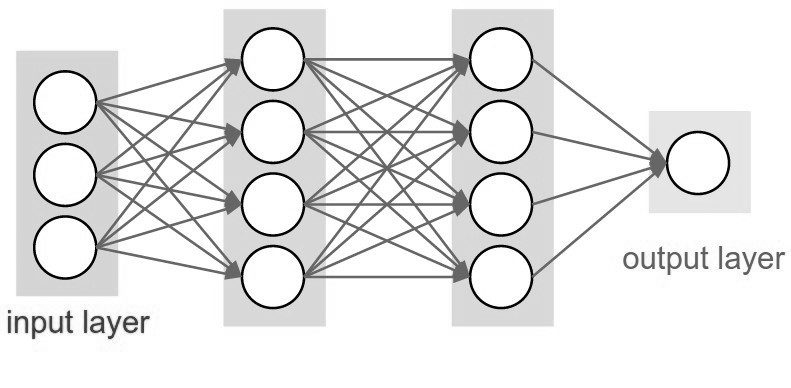
\includegraphics [width=0.7\textwidth] {o/neuralnetwork.png}
\caption{The basic structure of a neural network.}
\end{figure}
For example, let's consider the task of classifying handwritten digits, a task at which humans have traditionally outperformed automated methods.
The input  samples consist in a grayscale image of the written digits, so to each pixel in the image is associated a value from 0 to 1 proportional to the intensity of the image in that point.

Each neuron in the successive layer is a function (called the activation function) of a linear combinations of this input layer:
\begin{equation}
y_j(\textbf{x}, \textbf{w}) = f (\sum_i w_i x_i)
\end{equation}
As previously written, we hope that these neurons activate (e.g.
assume a high value) when certain global features are presented in the input furnished.
In the case of handwritten digits one of such features could be for example the presence of a loop, like in the digits zero, six, eight, nine, or the presence of a long vertical line, like in the digits one and four (see figure \ref{feat}).
In order to activate only when a long vertical line is present, it is necessary for the weights (also called "synapses strength" in analogy with biological neurons) in the linear combination that is the argument of the neuron to be big around the middle of the image, and negative or null in the remaining image.
\begin{figure} [H]
\centering
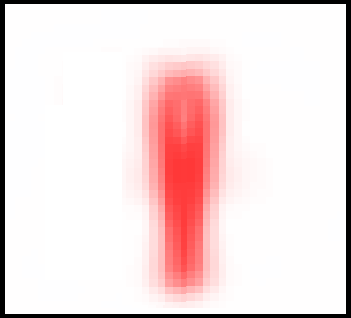
\includegraphics [height=4.5cm ,width=4.5cm ] {o/nine.png}
\caption{One of the features that we would want to extract from the original image.}
\label{feat}
\end{figure}
Then, in the successive layer, we want neurons to activate when a certain combinations of features is present.
For example, to distinguish a nine from the other digits, both a upper loop and a vertical line must be present.
So we would like one of these upper layer neurons to have a set of weights so that it activates if and only if both these features are present.

\begin{figure} [H]
\centering
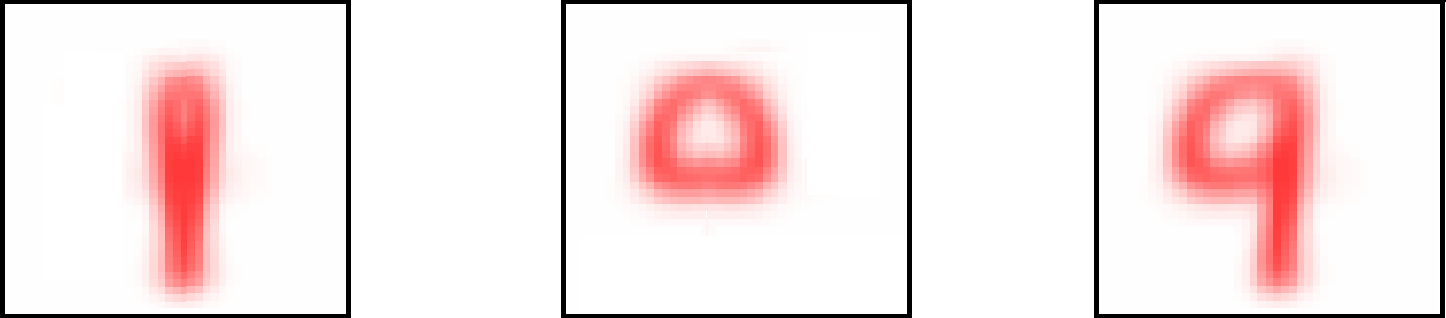
\includegraphics [width=\textwidth] {o/features.png}
\caption{In the image of a nine, both features are present.}
\end{figure}

As for the activation functions, one common example is the sigmoid:

\begin{equation}
	S(x) = \frac{1}{1+e^{-x}}.
	\label{sigmoid}
\end{equation}

\begin{figure}[H]
\centering
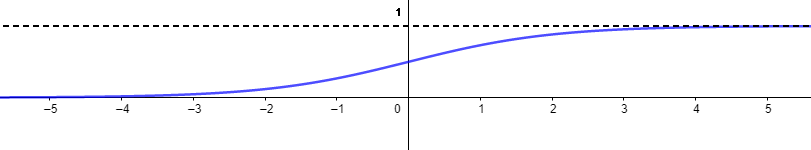
\includegraphics[width=\textwidth]{o/sigmoid.png}
\caption{Equation \ref{sigmoid}.}
\end{figure}
Which maps the real number range in the $[0,1]$ range, a property useful in network training to avoid a single neuron value overshadowing all other values.
Also, having all neurons assume a positive value is commonly a wanted feature of networks, and the same can be said of differentiability of the activation function.
Another common function used is the ReLU (rectified linear units):

\begin{equation}
	RelU(x) = max(0, x).
	\label{relu}
\end{equation}

\begin{figure}[H]
\centering
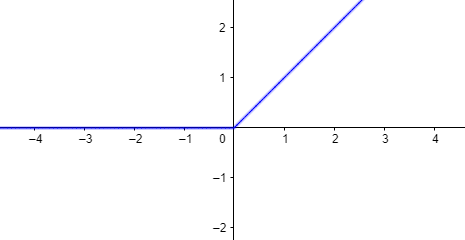
\includegraphics[height=5cm]{o/relu.png}
\caption{Equation \ref{relu}.}
\end{figure}

Which is differentiable and strictly positive, like the sigmoid.

The final output layer would be composed of ten neurons, of winch only one would activate for each digit.
For example, we would like the final output value to be one for the correct digit, and zero for all the others.
Note that we did not specified the number of neurons, as we do not know the number of features highlighted in any layer, nor we know what the optimal number of layer is.
Typically, a case-by-case judgement must be made, depending on the task we need to solve;
there is no global rule to define the number of neurons and layers.

Now let's discuss the problem of how effectively train the network so that its parameters have appropriate values.

\subsection{Network training}
At first, the weights of the network are randomly initialized, so naturally the goodness of classification is low.
In supervised learning (commonly used with neural networks) We first define a function, called error or loss function, that quantifies the error in the classification of the datasets.
For example, in our hypothetical network for the classification of digits, a common choice for the error function would be

\begin{equation}
f(x)=\frac{1}{2}||x-x_{true}||_2
\label{true}
\end{equation}
That is, half the square of the difference between the output vector and the correct output.
In this case, the correct output vector corresponds to one in the n-th dimension of the vector, where n is the digit represented by the input, and zero in all other dimensions.

Considering the space of all possible weights value, training the network reduces to finding the point of this space (that is, the set of weights) that minimizes this error function on the dataset.
This is obtained thought a technique known as gradient descent.
In gradient descent we calculate the gradient of the loss function, then we take consecutive steps in the opposite direction of the gradient to the minimum of the loss function.

\begin{figure}[H]
\centering
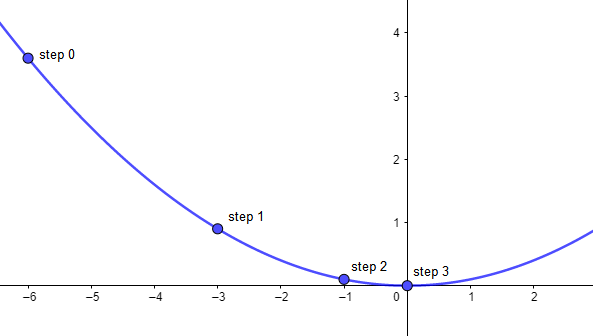
\includegraphics[height=6cm]{o/gradient.png}
\caption{Following the opposite direction of gradient will lead to the minimum, given that the function is convex.}
\end{figure}

Notice how this requires the error function to be differentiable.
But how does one calculate the gradient within respect to the weights of all the neurons that are not output neurons?

\subsection{Backpropagation}
Backpropagation is a useful technique used to obtain the gradient within respect to neurons in all layers.
It is called backpropagation because in our formula the error \textit{propagates backward} from upper-layer neurons errors, in contrast with the normal neuron activation in which information propagates forward.

Now let's calculate the backpropagation formula for a feed-forward network with arbitrary activation functions.

Consider a weight $w_{ij}$ related to the synapse gong from neuron $l_i$ to neuron $m_j$ , where layer $l$ precedes layer $m$.
Then defining
\begin{equation}
a_j = \sum_i w_{ij}l_i
\label{pizza}
\end{equation}
We have
\begin{equation}
m_j = h(a_j)
\label{pizza2}
\end{equation}
For some activation function $h$.

Our task is to explicit the derivative of the loss function $E$ within respect to $w_{ij}$.
We can apply the chain rule
\begin{equation}
\frac{\partial E}{\partial w_{ij}}=\frac{\partial E}{\partial a_j} \frac{\partial a_j}{\partial w_{ij}}.
\label{chain}
\end{equation}

Introducing the notation
\begin{equation}
    \delta_j = \frac{\partial E}{\partial a_j}
    \label{delta}
\end{equation}
Equation \ref{chain} becomes
\begin{equation}
	\frac{\partial E}{\partial w_{ij}} = \delta_j \frac{\partial a_j}{\partial w_{ij}}.
	\label{chain2}
\end{equation}
Deriving from \ref{pizza}
\begin{equation}
\frac{\partial a_j}{\partial w_{ij}} = l_i
\end{equation}
And substituting this result in \ref{chain2} we obtain
\begin{equation}
\frac{\partial E}{\partial w_{ij}}= l_i \delta_j
\end{equation}
We are almost done:
we just need to find a way to calculate the $\delta$ for each neuron in the network.

For the output layer units, this task is trivial.
For example, if the error function is defined as in \ref{true}, the $\delta$ for those neuron is
\begin{equation}
\delta_j = m_j - t_j
\end{equation}
Where $t_j$ is the expected output.

Since we have calculated $\delta$ for the last layer, we only need a formula to calculate $\delta$ for the neurons in a previous layer, and we will be able to calculate delta for all possible weights.
Applying the chain rule
\begin{equation}
\delta_j = \sum_k \frac{\partial E}{\partial a_k} \frac{\partial a_k}{\partial a_j}.
\end{equation}
Where $k$ is the successive layer were we already know the values of our $\delta$, we can substitute in equation \ref{delta}
\begin{equation}
\delta_j = \sum_k\delta_k \frac{\partial a_k}{\partial a_j}.
\end{equation}
And then using equation \ref{pizza} and \ref{pizza2}
\begin{equation}
\delta_j = \sum_k \delta_k \frac{\partial \sum_j w_{kj} h(a_j)}{\partial a_j}
\end{equation}
Which gives our final Backpropagation formula:
\begin{equation}
\delta_j = h'(a_j)\sum_k w_{jk}\delta_k.
\end{equation}

\todo[inline]{spiegare anche che ci sono problemi di convergenza numerica (nota: cioè?)}
\section{Biological plausibility of neural networks}
While a majority of papers on neural network in present-day literature are about supervised learning, a minority of articles exist referring to unsupervised learning.
In a 2019 paper by Dimitry Krotov and John J.
Hopfield is illustrated a unsupervised algorithm for training a neural network in an unsupervised fashion inspired by biological neural networks.
As we know, biology has inspired neural networks since the first steps in this direction of machine learning, and biological neural networks and artificial neural network have structural similarity, that is to say both are formed by layers of neurons greatly connected by synapses.
It should be noted that in most models of artificial neural networks these connections transmit information forward, while the human cortex for example presents backward, forward and lateral connection, whose functions are still to be fully understood.

The authors evidence two main biological implausibilities in artificial neural networks:
backpropagation techniques and supervised learning.

\subsection{Implausibility of supervised learning}

In the first months or years of their lives, newborn animals and humans central nervous system undergoes some type of long-type learning.
This learning is believed to be mostly unsupervised:
there are no labelled data and no specific task.
To use an analogy by D. Krotov, supervised learning would be like like teaching to newborns with flashcards, which is, as one can imagine, not a good idea.

\subsection{implausibility of backpropagation}
As we have seen in the backpropagation section, each $\delta$ can be calculated by the deltas of the previous layer, given that one knows all the weights and activations.

In multilayered networks, this means that in order to evaluate the infinitesimal evolution of a single network parameter one must know not only the current value of the weight and the activation of the two neurons connected by it, but also the activation value of all neurons in the layers above.

The algorithm is said to be non-local, requiring information from all the above layers.
In biological neural networks, by contrast the information available to a single synapse is only relative to the two cells it connects.
So the biological process is "local" in the sense that a synapse can evolve in any arbitrarily complicated function of some parameters, but in the end those parameters must be only those relative to the two cells it connects.
As we will see shortly, our algorithm is local in a less strict sense: in the sense that a synapse evolves only with the information of the layers it connects; no above layer information is used in its evolution.

\section{The algorithm}
In a 2019 paper, Dimity Krotov and John J. Hopfield proposed a neural network model whose main characteristics are unsupervised learning and locality of information.

The basic idea of the algorithm is to train a matrix of weights in a two layers network -in which one of the layers is our input layer.
Then the so trained matrix is used to transform the data, that is then meant to be classified with a supervised algorithm of some kind.
This makes the procedure not fully unsupervised, however we still retain the advantage of not needing a huge amount of labeled data for training, as the so processed data is more easily classified by the supervised part of the algorithm.

\subsection{Training}

The parameters of the network, corresponding to the scalars that compose the matrix, are trained using the gradient descent technique previously discussed, with a variation:

Processing the whole database at each step of training would be time consuming. Instead, using a technique known as \textit{stochastic} gradient descent, we take a subset of the database  (known as minibatch) and treat it as the whole database. Due to statistical fluctuations, the minibatch will obviously not be representative of the whole database: at a practical level, this means that the gradient we are calculating is not precisely in the direction of the actual gradient, the one that we would only get processing the whole database in a single minibatch. We are, however, trading a reasonable amount of precision for the possibility of processing way more batches that we would we able to if each batch was composed of the whole database, so in the end working in minibatches works in favor of our objective, that is reaching convergence to a set of trained weights able to make predictions on the testing database.

The authors also sum up the characteristics of the algorithm  in four points:
\begin{itemize}
	\item The change of synapse strength is proportional to the activity of the presynaptic cell and to a function of the activity of the postsynaptic cell.
	\item Lateral inhibition between patterns is present.
	\item Homeostatic constraints results in the strengths of the synapses of each hidden neuron converging to a sphere.
	\item The sphere is defined for a Lebesgue norm with $p \geq 2$.
\end{itemize}

The Lebesgue norm for a finite-dimensional vector is defined as

\begin{equation}
	||x||_p = (|x_1|^p+|x_2|^p+\cdots +|x_n|^p)^{1/p}
\end{equation}

Where $p$ is a real number bigger than one.
This definition reduces to the euclidean norm when $p=2$.

\begin{figure} [H]
\centering
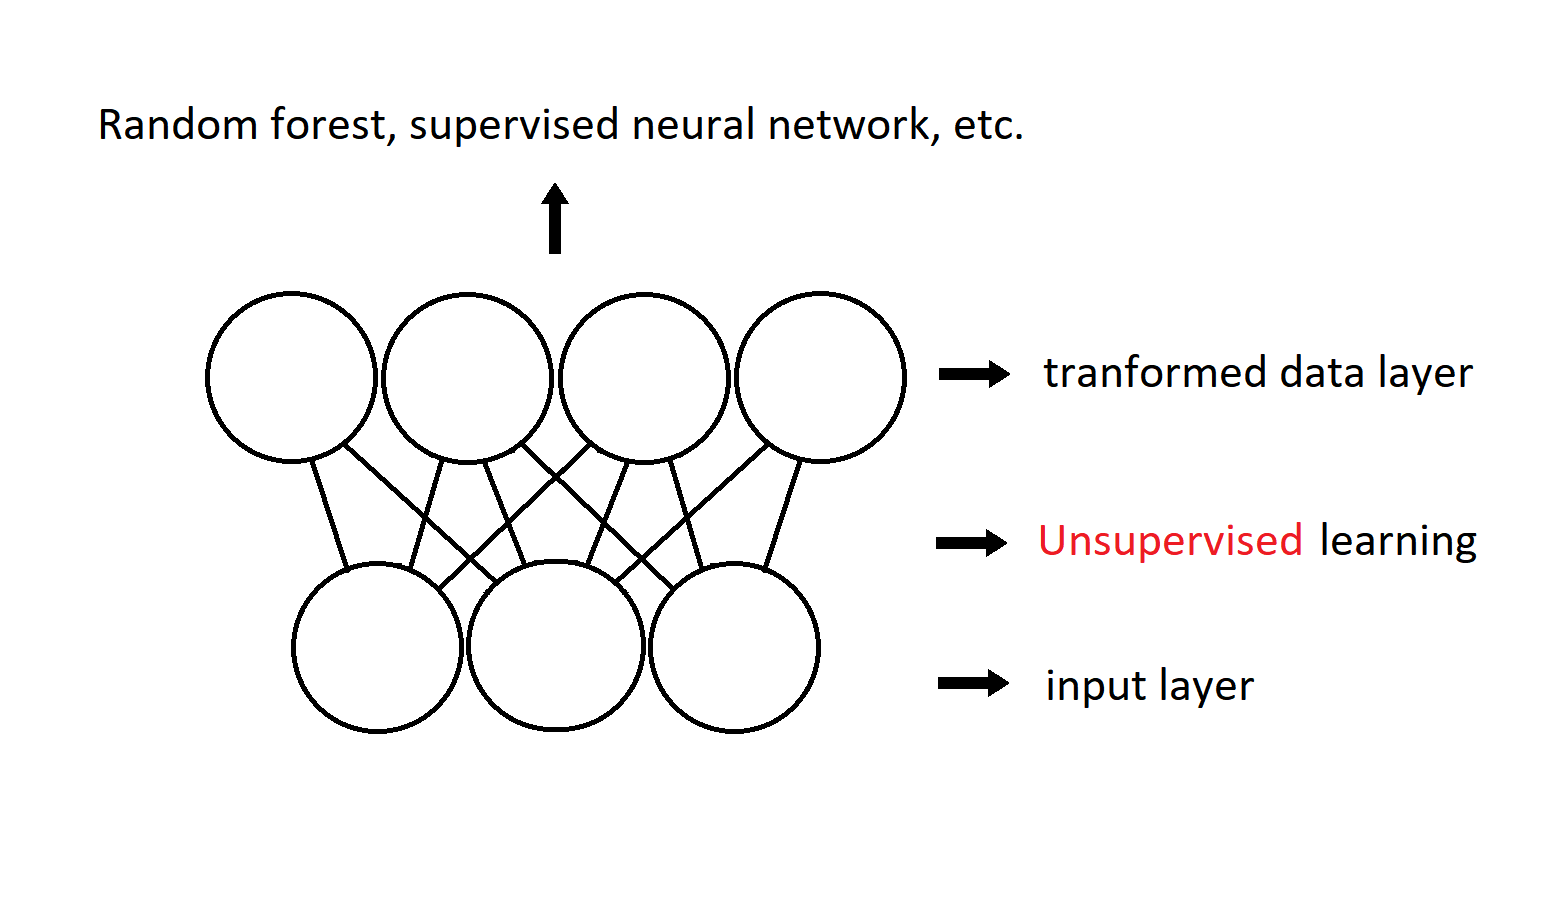
\includegraphics [height=7cm ,width=12cm ] {o/2parti2.png}
\caption{The structure of the model.}
\end{figure}

The main equation of the algorithm is

\begin{equation}
    \tau_L \frac{dW_{ij}}{dt} = g(h_i)(R^p v_i - \braket{\textbf{W,v}}_i W_{ij} )
    \label{main}
\end{equation}

Where

\begin{equation}
    \braket{\textbf{W,v}}_i = \sum_j W_{ij} |W_{ij}|^{p-2} v_j
\end{equation}

And $\tau_L$ is a time scale parameter,  $W_{ij}$ is the strength of the synapse connecting the i-th hidden neuron with the j-th input neuron, $h_i$ is the i-th hidden neuron, $R$ is the radius of the sphere at which the weights of the synapses of each hidden neuron will converge, $p$ is the Lebesgue norm exponent, $g(h_i)$ is a function that assumes value
\begin{itemize}
    \item $1$ if $h_i$ is the most-activated hidden neuron,
    \item $-\Delta$ if $h_i$ is the k-th most activated hidden neuron, where $\Delta$ and $k$ are parameters of the algorithm,
    \item and zero in all other cases.
\end{itemize}

As evaluating $g$ implies ranking all hidden neurons by activation, there's an implicit competition between patterns.
The cases in which has value of one and a negative value correspond to Hebbian and anti-Hebbian learning respectively.

Within regards to computational complexity, it was expected to be O(N) \todo[inline]{spiegare cosa sia la complessità computazionale}, where N is the number of epochs processed.
Trying five different values of N gave a linear correlation coefficient of 0.99, thus confirming a computational complexity of O(N).

\subsection{Purpose of this paper}

I reproduced the model, analyzing its behavior under various variations from the original, quantifying its prediction accuracy working on the MNIST handwritten digits database in conjunction with three different supervised algorithms used for classification purposes.

\subsection{Switching off explicit anti-Hebbian learning}

In about 20\% of cases the algorithm was observed converging to the pattern shown in figure \ref{nove}. \todo[inline]{fare riferimento a figure future è difficile da seguire (nota: l'alternativa è spostare questo paragrafo, diminuendo l'importanza di questa variante dell'algoritmo. dovrei farlo?)}
As one can imagine, this is not quite useful for classification:
in these cases the classification score lowered to around 20\% in all supervised learning scenarios.

A theoretical explanation can be attempted in terms of insufficient differentiation of initial synapses values, and this is confirmed by the fact that reducing the standard deviation makes this result consistent.
A single hidden neuron, the one that has only positive value at convergence, in the upper right corner of this image, is chosen as the most activated in a majority of cases, resulting in all the other neurons synapses values getting lowered.

To avoid this, a variation from the original algorithm has been implemented, switching off the negative reinforcement, and only keeping the positive reinforcement learning.
Note that this still maintains a form of competition between neurons, as only the most activated one gets updated at all.

Now the weights are only positive and strictly resemble prototypes of digits (figure \ref{nodelta}).
The accuracy of prediction is only minimally changed.
Another change observed is that now the weights actually converge to a sphere (figures \ref{uu_hist} and \ref{ii_hist})

\section{The MNIST database}

The Modified National Institute of Standards and Technology database is a set of images of handwritten digits. The images are grayscale-level, centered, size-normalized and have a resolution of 28 by 28 pixels images of handwritten digits.
The digits were written by 500 writers, United States Census Bureau employees and US high school students.

\begin{figure} [H]
	\centering
	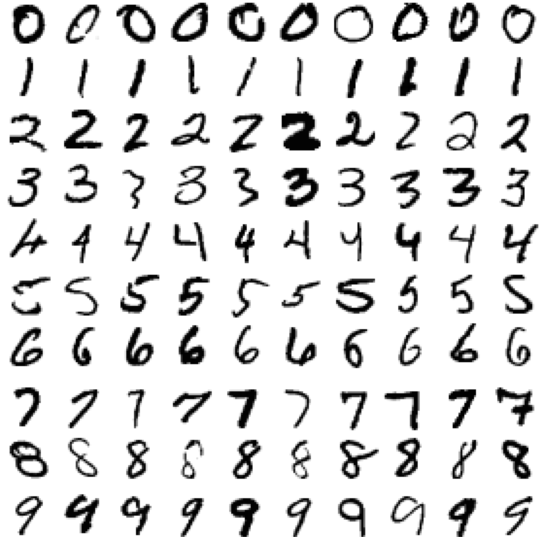
\includegraphics [width=7.5cm ] {o/mnist.png}
	\caption{Samples from the data set.}
	\label{mnist}
\end{figure}

The dataset is commonly used as a simple dataset for testing machine learning algorithms.
\chapter{Accuracy and visual characterization}

\section{Supervised phase}
Accuracy is defined the percentage of correctly classified samples.
It is, of course, not useful to test this quantification of our model's performance on the same database used to train our model.
For this reason, the database has been split in two:
a training database of 450,000 samples and a database for testing accuracy of 10,000 samples.
The sizes in which to subdivide the original datasets are not fixed, but the general rule is that the bigger the training dataset is, the better the accuracy.

To actually classify samples, we used three different supervised algorithms, to test on the data transformed with the weight matrix trained with our algorithm.

\subsection{Random forest}
The random forest is a supervised machine learning method that is based on a set of random trees, a simpler classification method.

\subsubsection{Decision trees}
 At its core, a decision tree is nothing more than a set of binary decisions based on data associated with the samples.
The data can be both categorical (i.e.  it is a true of false affirmation) or numerical (i.e.  it has a value associated to it), in which case we make use of thresholds to turn use it as if it was categorical.
(see figure \ref{chestt})

\begin{figure} [H]
    \centering
    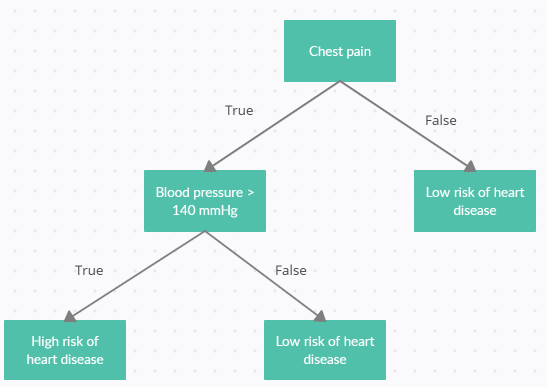
\includegraphics [width=12cm] {o/chestt.png}
    \caption{An example of a decision tree.}
    \label{chestt}
\end{figure}

This is the basic structure of decision trees.
Realistic decision trees have much more nodes (The decisions that need to be taken) and leaves (The final classifications).
Note that a tree can ask for the same numerical data to pass or not more than one different threshold (for example, a tree could ask if a patient heart is over 60 bpm and later down the stream ask if the heart rate is over 80 bpm).

\subsubsection{Building decision trees}

So, in order to classify our data, we need to choose thresholds for the numerical values in the features of our samples, then choose the right order of the question nodes, and then assign a label to each leaf in the tree.
Let's see the main concept that allows us to do this:
the Gini impurity.
It is an indicator of how good a single feature is at classifying our data.
The Gini impurity equals

\begin{equation}
    G = \sum_i p(C_i) \cdot (1 - p(C_i))
\end{equation}

Where $p(C_i)$ is the probability of a sample belonging to class $C_i$.
The lower the Gini impurity is, the better that single feature is a separating data by class.
A feature that perfectly classifies the whole database has a Gini impurity of 0.

For example, let's consider this toy database:

\begin{table}[H]
  \begin{center}
    \begin{tabular}{c|c|c} % <-- Alignments: 1st column left, 2nd middle and 3rd right, with vertical lines in between
      \textbf{Blood pressure} & \textbf{Risk of hearth disease}\\
      \hline
      Patient 1 &  176 mmHg & High\\
      Patient 2 &  168 mmHg & High\\
      Patient 3 &  153 mmHg & High\\
      Patient 4 &  145 mmHg & High\\
      Patient 5 &  136 mmHg & Low\\
      Patient 6 &  127 mmHg & High\\
      Patient 7 &  125 mmHg & Low\\
      Patient 8 &  119 mmHg & Low\\
      Patient 9 &  118 mmHg & Low\\
    \end{tabular}
    \caption{Toy database: blood pressure and risk of hearth disease as evaluated by a medical professional.}
    \label{tree_table}
  \end{center}
\end{table}


of 4 patients with blood pressure above 140 mmHg that are at a high risk for heart disease, 1 patient with blood pressure below 140 mmHg that is at a high risk for heart disease, and 5 patients with blood pressure below 140 mmHg, at low risk for heart disease (Note that in order to perform this kind of learning each sample in our training database must already be correctly labelled, as random trees are a form of supervised learning ).
Given this database, how good is a blood pressure threshold at 140 mmhg at classifying our patients in high or low risk of heart disease?
Calculating the Gini impurity for the unsplit database gives us

\begin{equation}
    G = 0.5 \cdot 0.5 + (1-0.5) \cdot (1-0.5) = 0.5
\end{equation}

Now let's split the database at our give threshold and calculate the Gini impurity for only patient with a blood pressure bigger than 140 mmHg

\begin{equation}
    G_{high} = 0 \cdot (1 -0) + 1 \cdot (1-1) = 0
\end{equation}

And for patients with a lower than 140 mmHg blood pressure

\begin{equation}
    G_{low} = \frac{1}{6} \cdot (1 - \frac{1}{6}) + \frac{5}{6} \cdot (1- \frac{5}{6}) = 0.278.
\end{equation}

And now we evaluate the averaged Gini impurity

\begin{equation}
    G_{split} = \frac{4}{10} \cdot G_{high} + \frac{6}{10} \cdot G_{low} = 0.167
\end{equation}

So now we know that applying the split reduces the Gini impurity from 0.5 to 0.167.

Getting back to the problem of actually building the decision tree, we first decide the best threshold for each numerical feature by calculating the Gini impurity for each value, then we build the tree starting with the feature that lowers the impurity the most.
During our descent long the tree, if we ever find a node were subsequential splitting can only increase the Gini impurity, we stop there and make the node a leaf.

\subsubsection{Building random forests}
Random trees, while easy to build, interpret and implement, as a method for supervised learning are (sadly) hindered by the low accuracy that characterizes this method.
By their own nature they are very sensible to outliers. The reason for this can be understood by looking at their hierarchical nature: a single split that is not very good propagates this error downstream.\todo[inline]{giustificare! citazioni, esempi, etc\ldots}

Random forests are a method for adding flexibility to decision trees.
A random forest is a set of decision trees in which classification is given by a majority vote from all trees.
To build a random forest, the first step is to perform bootstrap aggregating (or "bagging") on the dataset, that is, to take randomly with replacement from the dataset to build a second, "bagged" dataset.
The second step is to build a decision tree from the bagged dataset, but with a difference:
at each step in building the tree, only a subset of variables is considered.
Then the process is repeated until we have a considerable number of trees, the random forest;
The two expedients we have used in building the trees, using a bagged dataset and only considering a subset of variables at each step, allow us to have greater flexibility and less sensitivity to outliers.

\begin{figure} [H]
\centering
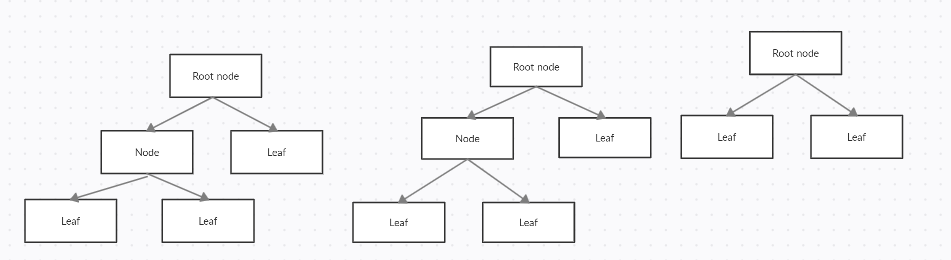
\includegraphics [width=\textwidth ] {o/forest.png}
\caption{An example of a random forest model composed by three trees.}
\label{forest}
\end{figure}

\subsection{Support vector machines}

The second method used for the supervised learning of the algorithm, the Support vector Machine or SVM, a common and robust method for classification.

Suppose that our training database is composed of data that is separable by a hyperplane in the space of features.

An hyperplane is a set of $\textbf{x}$ points satisfying

\begin{equation}
    \textbf{w}^T\textbf{x} -b = 0
\end{equation}

For a certain vector $\textbf{w}$ normal to the plane and for a certain scalar $b$, So that data on one side of the plane belongs to one class and data to the other side belongs to the other.
Note that we can easily generalize for multiclass problems reducing the to multiple one-vs-all binary classification problems.
The problem is of course to find the right parameters to correctly place the hyperplane.

\begin{figure} [H]
    \centering
    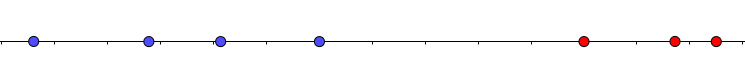
\includegraphics [width=\textwidth ]{svm/1dim.png}
    \caption{One-dimensional data samples divided in two classes.}
    \label{1dim}
\end{figure}


Our first approximation is to choose the plane so that it is equidistant from the two closest samples from each class.
This allows us to maximise the margin of space between every class and the hyperplane, which intuitively should in turn minimize misclassification.
For this reason, this technique is known as maximal margin classifier, while the points on the edge of the margin are called support vectors, from which support vector machine take name.

\begin{figure} [H]
    \centering
    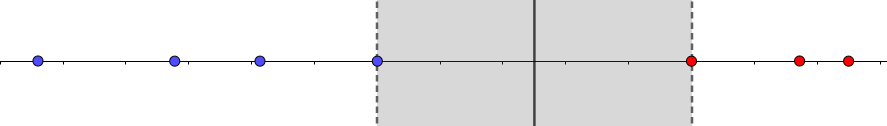
\includegraphics [width=\textwidth ]{svm/1dim_disq.png}
    \caption{Picking a hyperplane equidistant from the two nearest points least to the biggest margins possible. With monodimensional data, a hyperplane corresponds to a single point.}
    \label{1dim1_disq}
\end{figure}

However, this choice is far from the ideal one.
Our model has very poor flexibility:
even just one outlier can create great imprecision (figure \ref{1dim_disq2})


\begin{figure} [H]
    \centering
    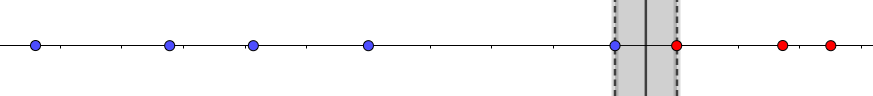
\includegraphics [width=\textwidth ]{svm/1dim_disq2.png}
    \caption{A single outlier can greatly reduce the margin.}
    \label{1dim_disq2}
\end{figure}

In figure \ref{1dim_disq2}, one would classify any new samples on the left of the maximal margin as belonging to the class whose points are represented in violet, but intuitively we would like to assign the to the other class instead.

To remedy for this, we must allow for misclassification to take place.
By allowing our model to misclassify samples in a certain number (figure \ref{1dim_alw}) we are making the model less responsive of the training data but more flexible in classifying new samples.
A balance between these two characteristics must be found model by model.

\begin{figure} [H]
    \centering
    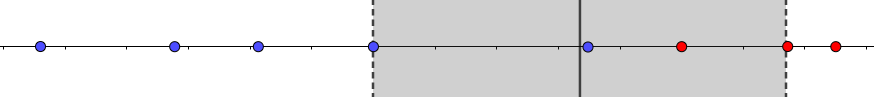
\includegraphics [width=\textwidth ]{svm/1dim_alw.png}
    \caption{Allowing for a certain number of  misclassifications improves the model.}
    \label{1dim_alw}
\end{figure}

Support vector machine can, of course, be generalized to non-linearly separable data:
it is very rare for a dataset to be linearly separable, so a model that only works in that case would be barely useful.
It can be done by transforming the data into higher dimensions, associating to each to these higher dimension parameters a value based on the original parameters of each sample.
For example, in figure \ref{2dim} the transformation is $x \xrightarrow{}(x,x^2)$.
Then the decision boundary will be a hyperplane in this higher dimensional space.
The transformation $x \xrightarrow{} (x, x^2, x^3, ...)$ is a common choice known as polynomial kernel transformation, but many more transformations can be useful depending on the data.

\begin{figure} [H]
    \centering
    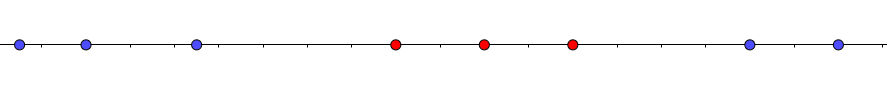
\includegraphics [width=\textwidth ]{svm/1dim_ns.png}
    \caption{Non linearly separable monodimensional data.}
    \label{1dim_ns}
\end{figure}

\begin{figure} [H]
    \centering
    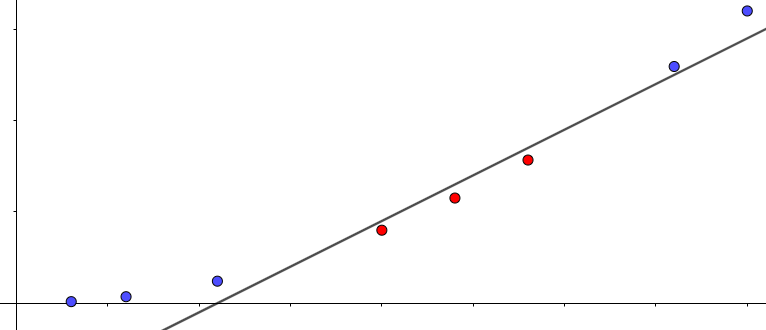
\includegraphics [width=\textwidth ]{svm/2dim.png}
    \caption{shifting the data to higher dimensions can make it linearly separable.}
    \label{2dim}
\end{figure}

A key point to take into consideration is that adding new dimensions can rapidly make the computational costs infeasible: as one can imagine, when operating on realistic database the number of dimensions that one needs to add to make the data separable can be very big.
Fortunately, there is a way to operate the calculations needed without never actually calculating the values of these extra dimensions for each sample.

Let $\phi (x)$ be the function that transposes in higher dimension our samples $x$. It is possible to express the equation that allows us to calculate the best separation hyperplane $W$ only as a function of the matrix $K$:
\begin{equation}
K =
	\begin{bmatrix}
		\phi (x_1) \phi(x_1)^T & \ldots & \phi (x_1) \phi(x_n)^T \\
		\ldots                 & \ldots & \ldots \\
		\phi (x_n) \phi(x_1)^T & \ldots & \phi (x_n) \phi(x_n)^T
	\end{bmatrix}
\end{equation}	

Where $\phi$ is the transformation in higher dimensions of our samples.

Now, Mercer's theorem states that such a matrix, being symmetrical and positive semidefinite, can be expressed as a function of $x$ without explicitly calculating $\phi (x)$: 

\begin{equation}
K =
\begin{bmatrix}
	k(x_1, x_1) & \ldots & k(x_1, x_n) \\
	\ldots                 & \ldots & \ldots \\
	k(x_n, x_1) & \ldots & k(x_n, x_n)
\end{bmatrix}
\end{equation}

For example, consider this transformation from 2 to 3 dimensions:

\begin{equation}
	\phi (x_1, x_2) = (x_1^2, \sqrt 2 x_1x_2, x_2^2)
\end{equation}

The dot product between the vectors transposed to three dimensions with this transformation can be expressed as

\begin{equation}
	\phi(\textbf{x}) \cdot \phi(\textbf{y}) = x_1^2y_1^2 + 2x_1x_2y_1y_2 + x_2^2y_2^2 = (x_1y_1+x_2y_2)^2 = (\textbf{x} \cdot \textbf{y})^2.
\end{equation}

\todo[inline]{deve spiegare più nel dettaglio il metodo che ha implementato, quasi non c'è per nulla la spiegazione!}

\section{Accuracy table}

Now that we have explained the three supervised methods (The supervised network is explained in the introduction) used in conjunction with our algorithm we can see the accuracy reached with all three methods, where accuracy is defined as the percentage of correctly classified samples of our 10,000 samples testing database.

\begin{table}[h!]
  \begin{center}
    \begin{tabular}{c|c|c} % <-- Alignments: 1st column left, 2nd middle and 3rd right, with vertical lines in between
      \textbf{Method} & \textbf{Without unsupervised learning} & \textbf{With unsupervised learning}\\
      \hline
      Random forest & 96.90  ± 0.02 & 92.91 ± 0.04\\
      Supervised network & 90.0 ± 0.2 & 89.4 ± 0.3 \\
      SVM & 90.3 ± 0.1 & 91.6 ± 0.3 \\
    \end{tabular}
  \end{center}
  \caption{Accuracy of prediction of three supervised methods. Percentage of corrected guesses are reported in the central and right columns.}
  \label{bbb}
\end{table}

\subsection{Observations on table \ref{bbb}}

\begin{itemize}
    \item Preprocessing the data with the method illustrated led to mixed results, with the accuracy decreasing in the case of the random forest and the supervised network and increasing in the case of the support vector machine.
    \item In both columns, the random forest performs the best, and the supervised network the worst.
    \item Uncertainty on the accuracy is worse for all rows, as the algorithm adds another layer of random deviations to the network.
\end{itemize}

The literature standards for the accuracy reported in classifying the MNIST database digits are typically higher, around 95\%.
It is to be noted, however, that while the original paper by Hopfield and Krotov reaches a comparable accuracy, it does so with a number of second-layer neurons and epochs processed one order of magnitude higher than the algorithm discussed in this paper (2.000 neurons vs 100 and 1.000 epochs vs 100).
A point of strength of this model is the interpretability of the synapses:
we know that out of the one hundred neurons most of them resemble the prototype of a digit (see next section) and can thus act as a binary switch that confirms to the supervised part of the algorithm if the given input does or does not belong to a certain class.
This would seem to work best when working in conjunction with a random forest since it also works with a system of binary classification.
It is peculiar that instead, we observe a drop in accuracy when using the method in conjunction with the random forest.

\section{Visual characterization of patterns}
\todo[inline]{questi sono i risultati del modello originale di hopfield? non è chiaro}


\begin{figure} [H]
    \centering
    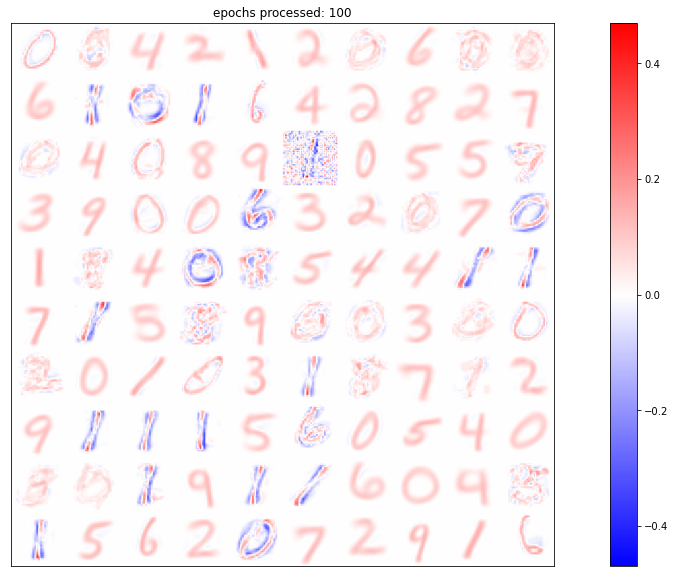
\includegraphics [width=12cm ] {h/uu_heatmap.png}
    \caption{A visual representation of the weight matrix, randomly initialized.There are one hundred hidden neurons, each of which has seven hundred eighty seven synapses, one for each pixel of the input, similarly arranged in a twenty eight by twenty eight matrix.}
    \label{heatmap}
\end{figure}

\subsection{Weight matrix: visual observations}

\begin{itemize}
    \item If we confront the emerging patterns in figure \ref{heatmap} with some samples randomly extracted from the dataset (figure \ref{mnist}), We can see that the emerging patterns resemble quite well the original digits. However, they are not a simple copy. For instance, in some cases negative values are present, while the original samples are all positive. From a mathematical standpoint, this is due to anti-Hebbian learning, in which weights are pushed away from a specific pattern.
    \item Patterns are also significantly different from those emerging in backpropagation-based neural networks (\ref{backnet}).
    \item All ten digits are present. There are other recurring patterns called "chromosome" and "six-pointed". Statistical frequencies are shown in graph \ref{cerchio1}. \todo[inline]{spiegare quali siano queste forme\ldots chi le ha definite, lei o hopfield?}
    \item Some patterns did not converge to something recognizable. An example is the synapses in the third row, fifth column of figure \ref{heatmap}.
    \item many zeros appear to be bordered in negative (blue) values. No other negative-encircled digits were observed in three different runs aside from the six in figure \ref{heatmap}, fourth row, fifth column.
    \item A chi square test was performed, validating the hypothesis of all digits being equally represented with $p  = 0.025$.
    \end{itemize}

\begin{figure} [H]
    \centering
    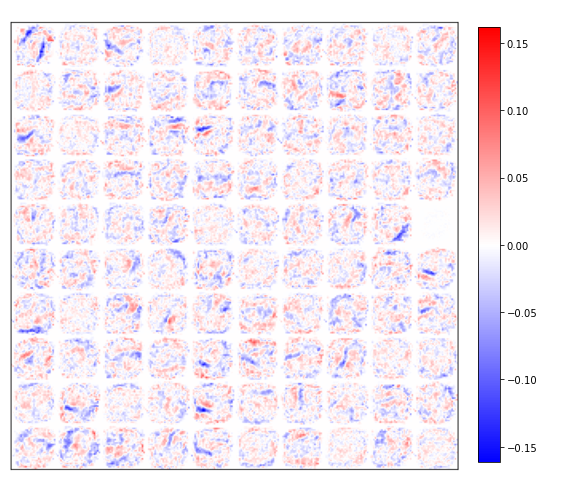
\includegraphics [width = 12cm] {h/backnet.png}
    \caption{Emerging pattern in a backpropagation network. \todo[inline]{manca contesto, questi sono i risultati per la rete neurale anche in input?}}
    \label{backnet}
\end{figure}

\begin{figure} [H]
    \centering
    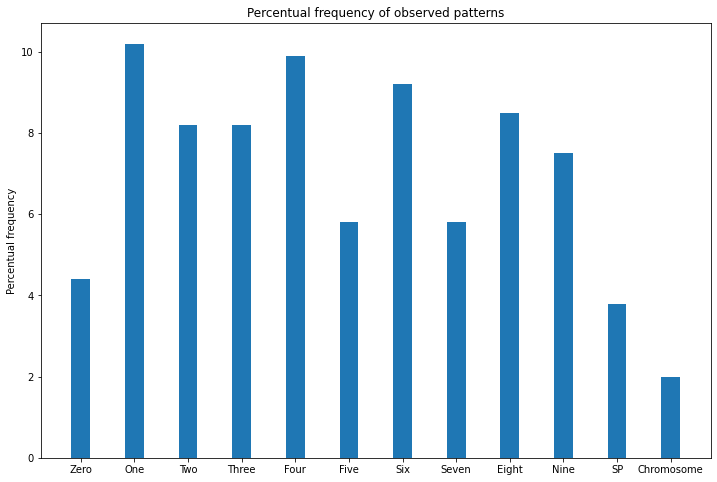
\includegraphics [width=12cm ] {o/bar2.png}
    \caption{Statistical frequency of observed patterns \todo[inline]{ottenuti con che metodo?}, recorded over three different training runs. An example of \textit{Six-pointed} (SP) pattern can be found in image \ref{heatmap}, row 2, column 2, while an example of \textit{Chromosome} pattern can be found in row 5, column 9. A chi-square test has been performed, accepting the null hypothesis with $p =0.025$.}
    \label{cerchio1}
\end{figure}

 Convergence to a sphere was not achieved:
in the observed behaviour was that some weights would always remain above the range of convergence \todo[inline]{quale sarebbe questo range?}, no matter the number of epochs (see figure \ref{uu_hist}).
However it was achieved when anti Hebbian learning was turned off (see figure \ref{ii_hist})
\begin{figure} [H]
    \centering
    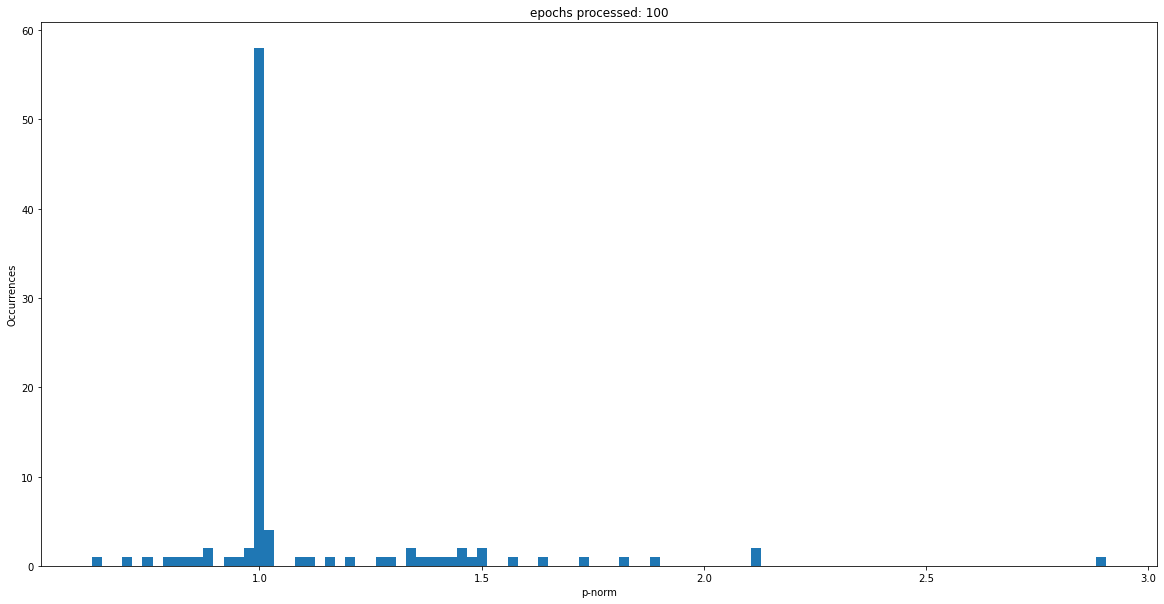
\includegraphics [width=12cm ] {o/uu_hist.png}
    \caption{Histogram of the p-norms of weight vectors for each hidden neuron.}
    \label{uu_hist}
\end{figure}

\begin{figure} [H]
    \centering
    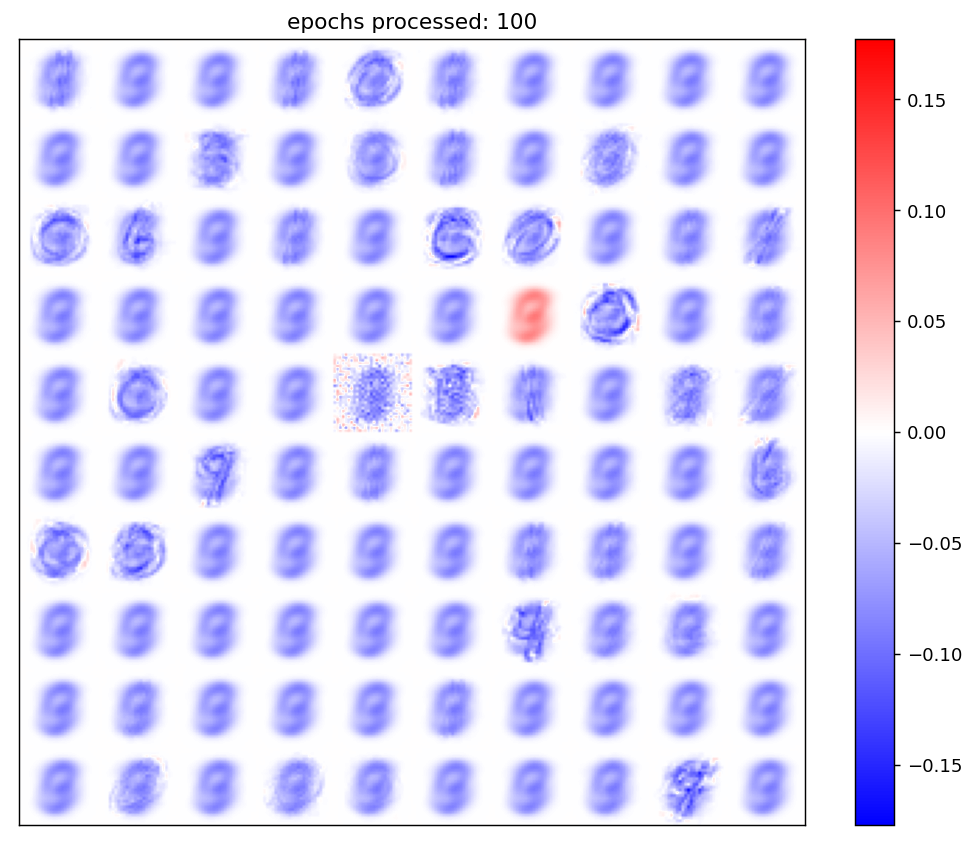
\includegraphics [width=12cm ] {h/nove.png}
    \caption{The pattern of convergence observed in 20\% of runs.}
    \label{nove}
\end{figure}

\begin{figure} [H]
    \centering
    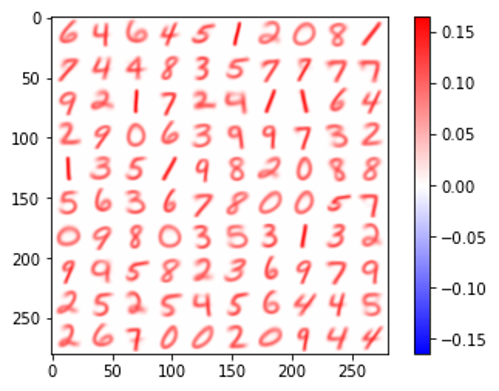
\includegraphics [width=12cm ] {h/nodelta.png}
    \caption{The pattern of convergence when explicit anti-Hebbian learning is turned off.}
    \label{nodelta}
\end{figure}

\subsection{Anti-Hebbian learning turned off: Observations}

\begin{itemize}
    \item Now all sets of synapses resemble prototypes of digits.
    \item A chi square test was performed, validating the hypothesis of all digits being equally represented with $p  = 0.025$.
    \item All weights are positive, as expected since values can only go up during learning.
\end{itemize}

In the original paper by Hopfield and Krotov this modification is tested, giving slight worse prediction results.
While the prediction results were only minimally changed in our implementation of the algorithm, it is interesting that the digits are now prototypes of digits with all digits represented (see figure \ref{o/cerchio2}).
These figures appear to be consistent, reappearing unchanged at modifications of various parameters of the algorithm, and are also very similar to the ones appearing in the "Exponential decay over time modification" and "Multiple neurons reinforced" modification (see sections with the same names in the chapter "Behaviour of variants", and in particular figures \ref{decay} and \ref{multiple}).

\begin{figure} [H]
    \centering
    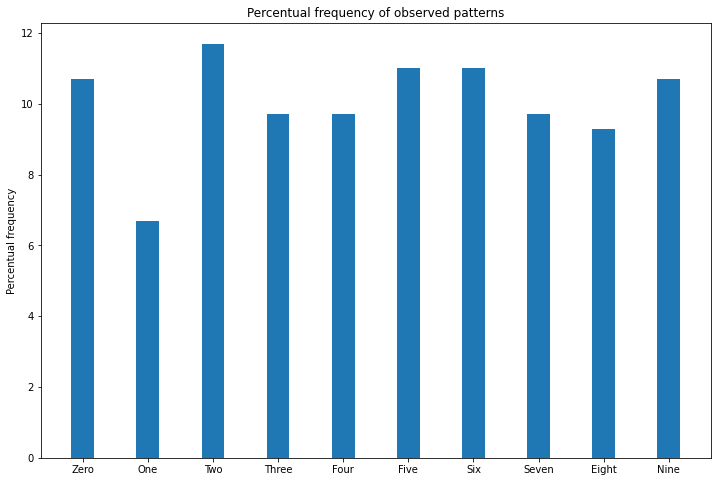
\includegraphics [width=12cm ] {o/bar1.png}
    \caption{Statistical frequency of observed patterns, recorded over three different training runs. Anti-Hebbian learning is turned off. An example of this con be seen in figure \ref{nodelta}. A chi-square test has been performed, accepting the null hypothesis with $p  = 0.025$.}
    \label{o/cerchio2}
\end{figure}
\begin{figure} [H]
\centering
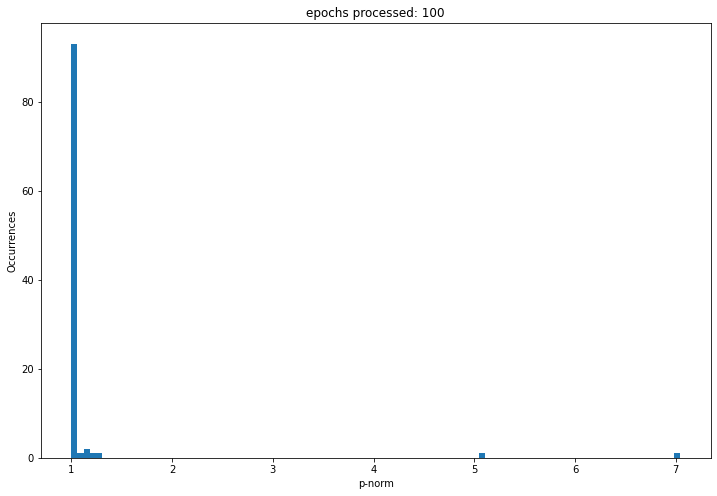
\includegraphics [width=12cm ] {o/ii_hist.png}
\caption{Histogram of the p-norms of weight vectors for each hidden neuron. Explicit anti-Hebbian learning is turned off. \todo[inline]{manca un commento nel testo}}
\label{ii_hist}
\end{figure}

\chapter{Behaviour of variants}

\section{Different batch compositions}

Another point of interest in the study of the model proposed was modifying the subdivision in batches of the database.
Two variations were used:
one in which the single batches were formed of only one digit, (figure \ref{monotype}) and one in which the batches were formed of two types of digits only (figure \ref{1v1}).

While this was expected to produce different patterns in synapses, both the patterns and the prediction accuracy did not change significantly.

\begin{figure} [H]
    \centering
    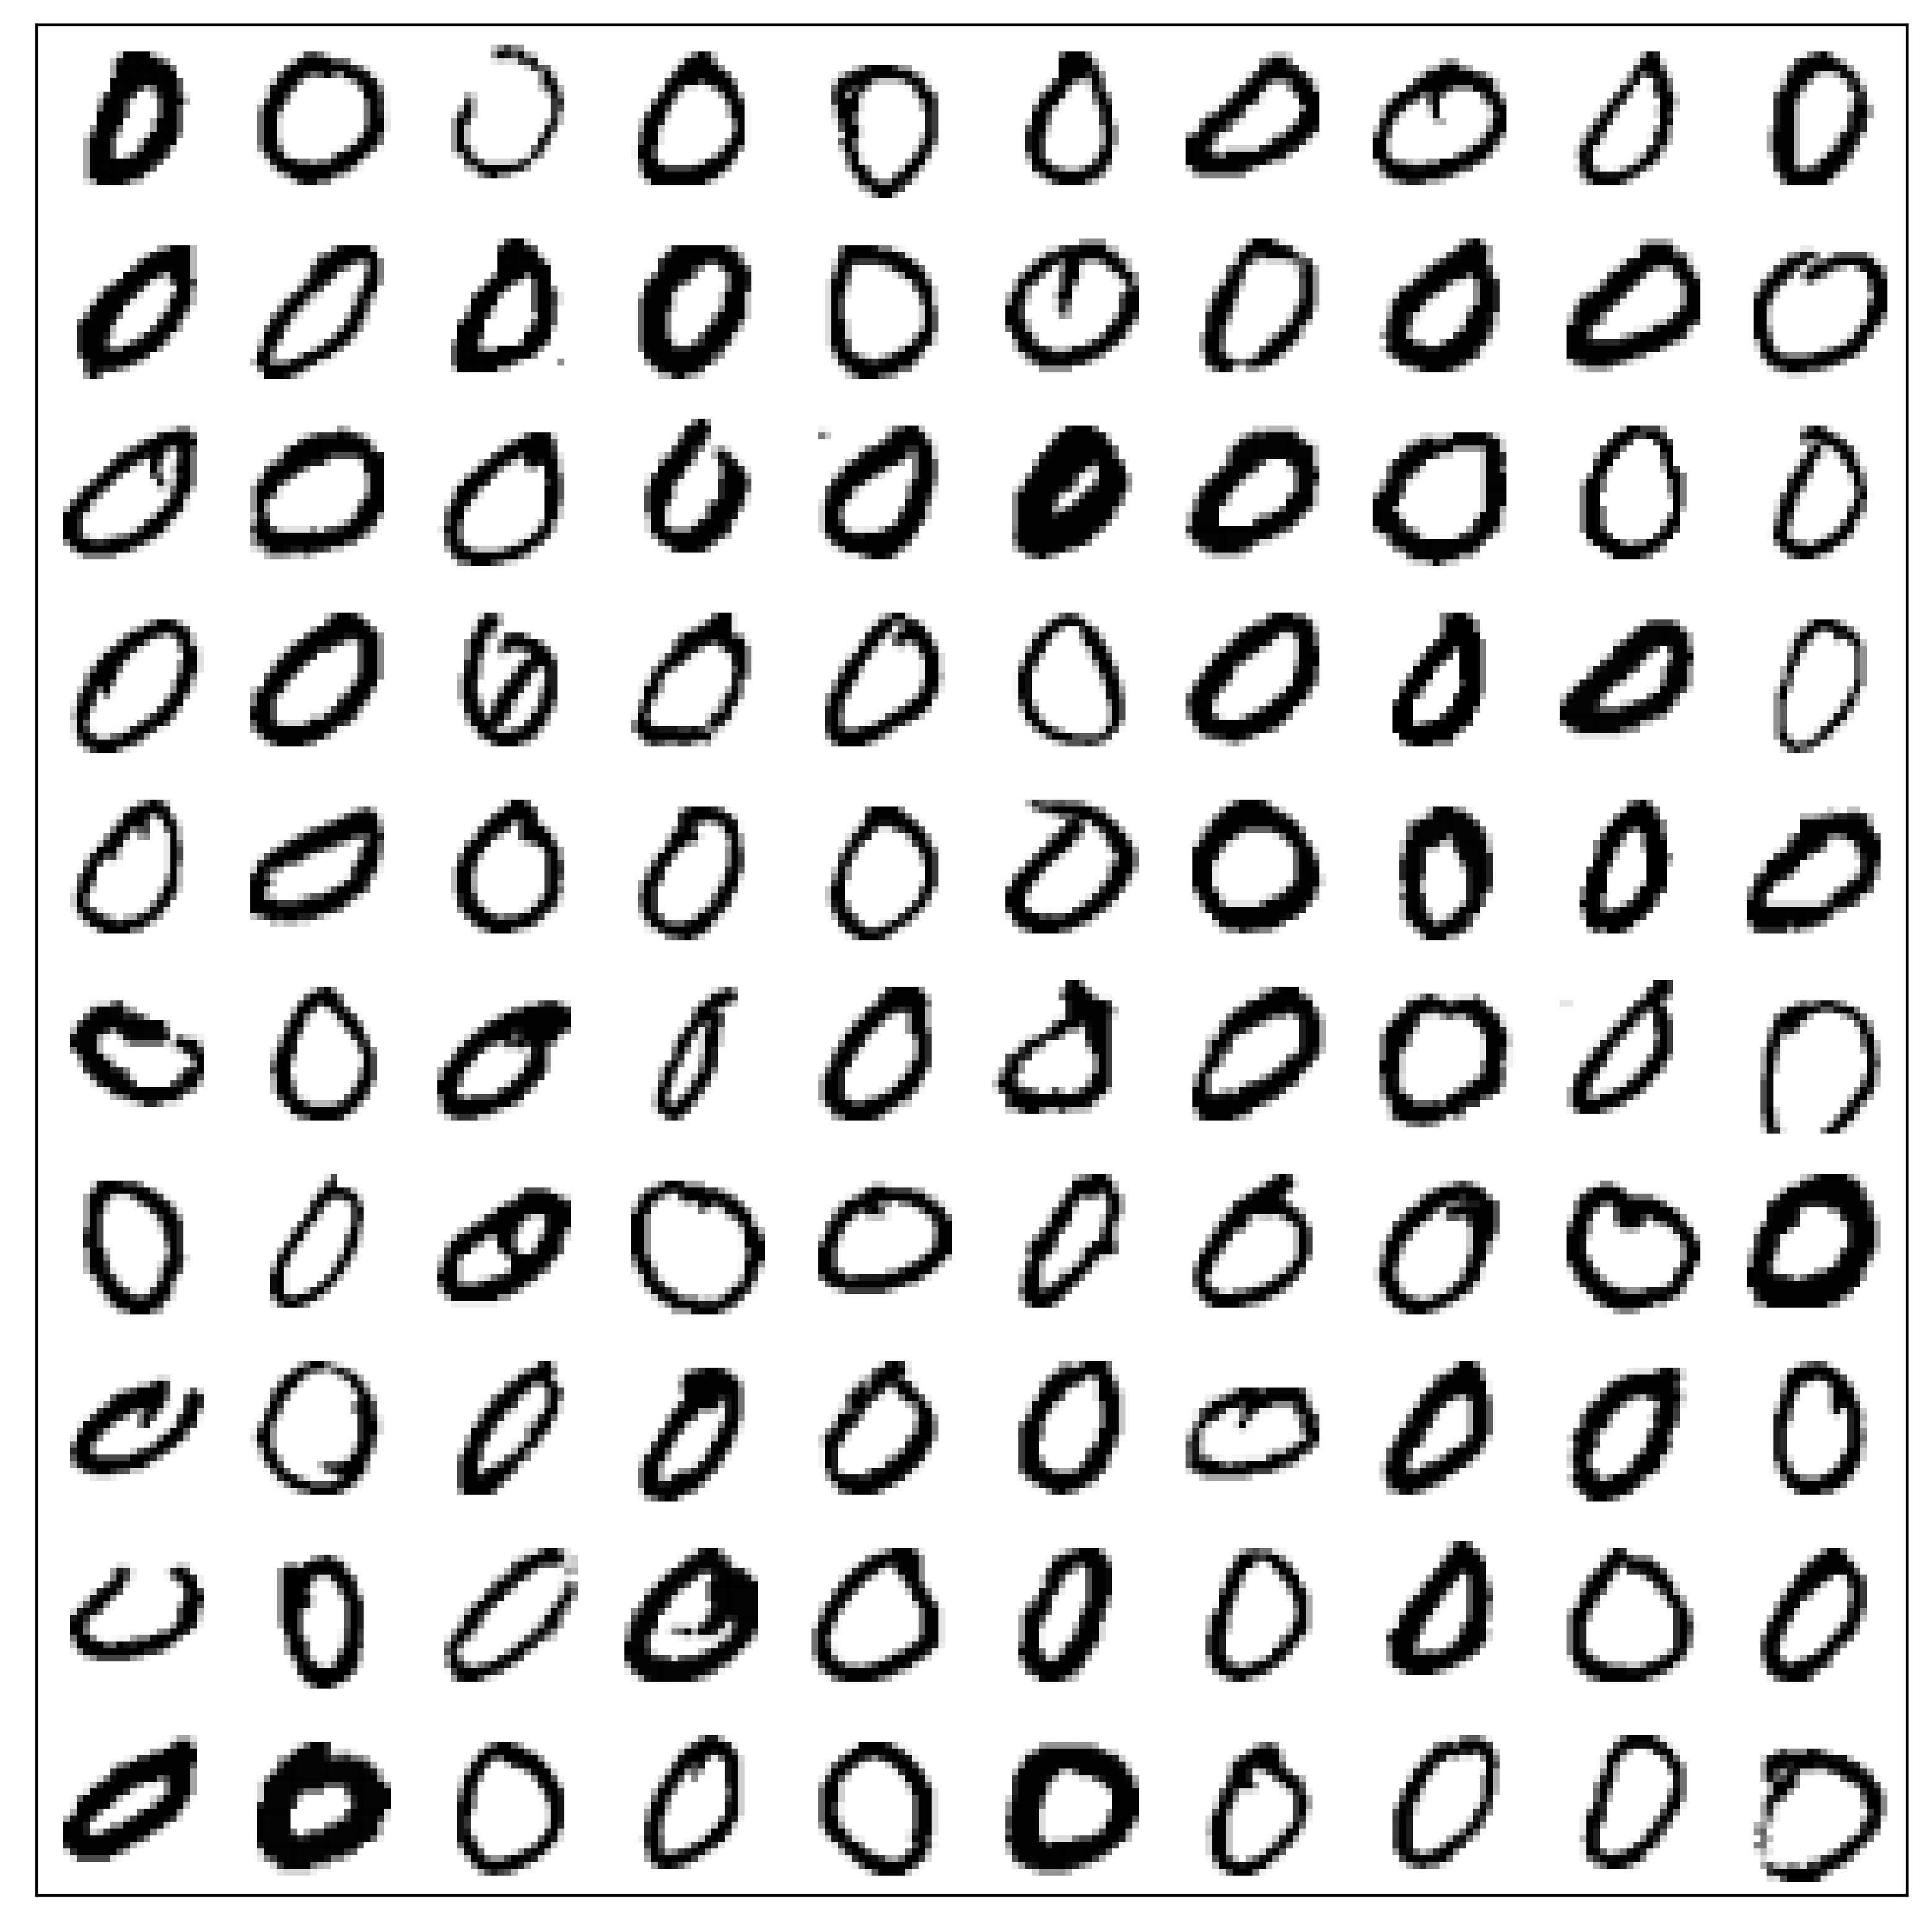
\includegraphics [width=10cm ] {o/0.png}
    \caption{"Monotype" batch example}
    \label{monotype}
\end{figure}

\begin{figure} [H]
    \centering
    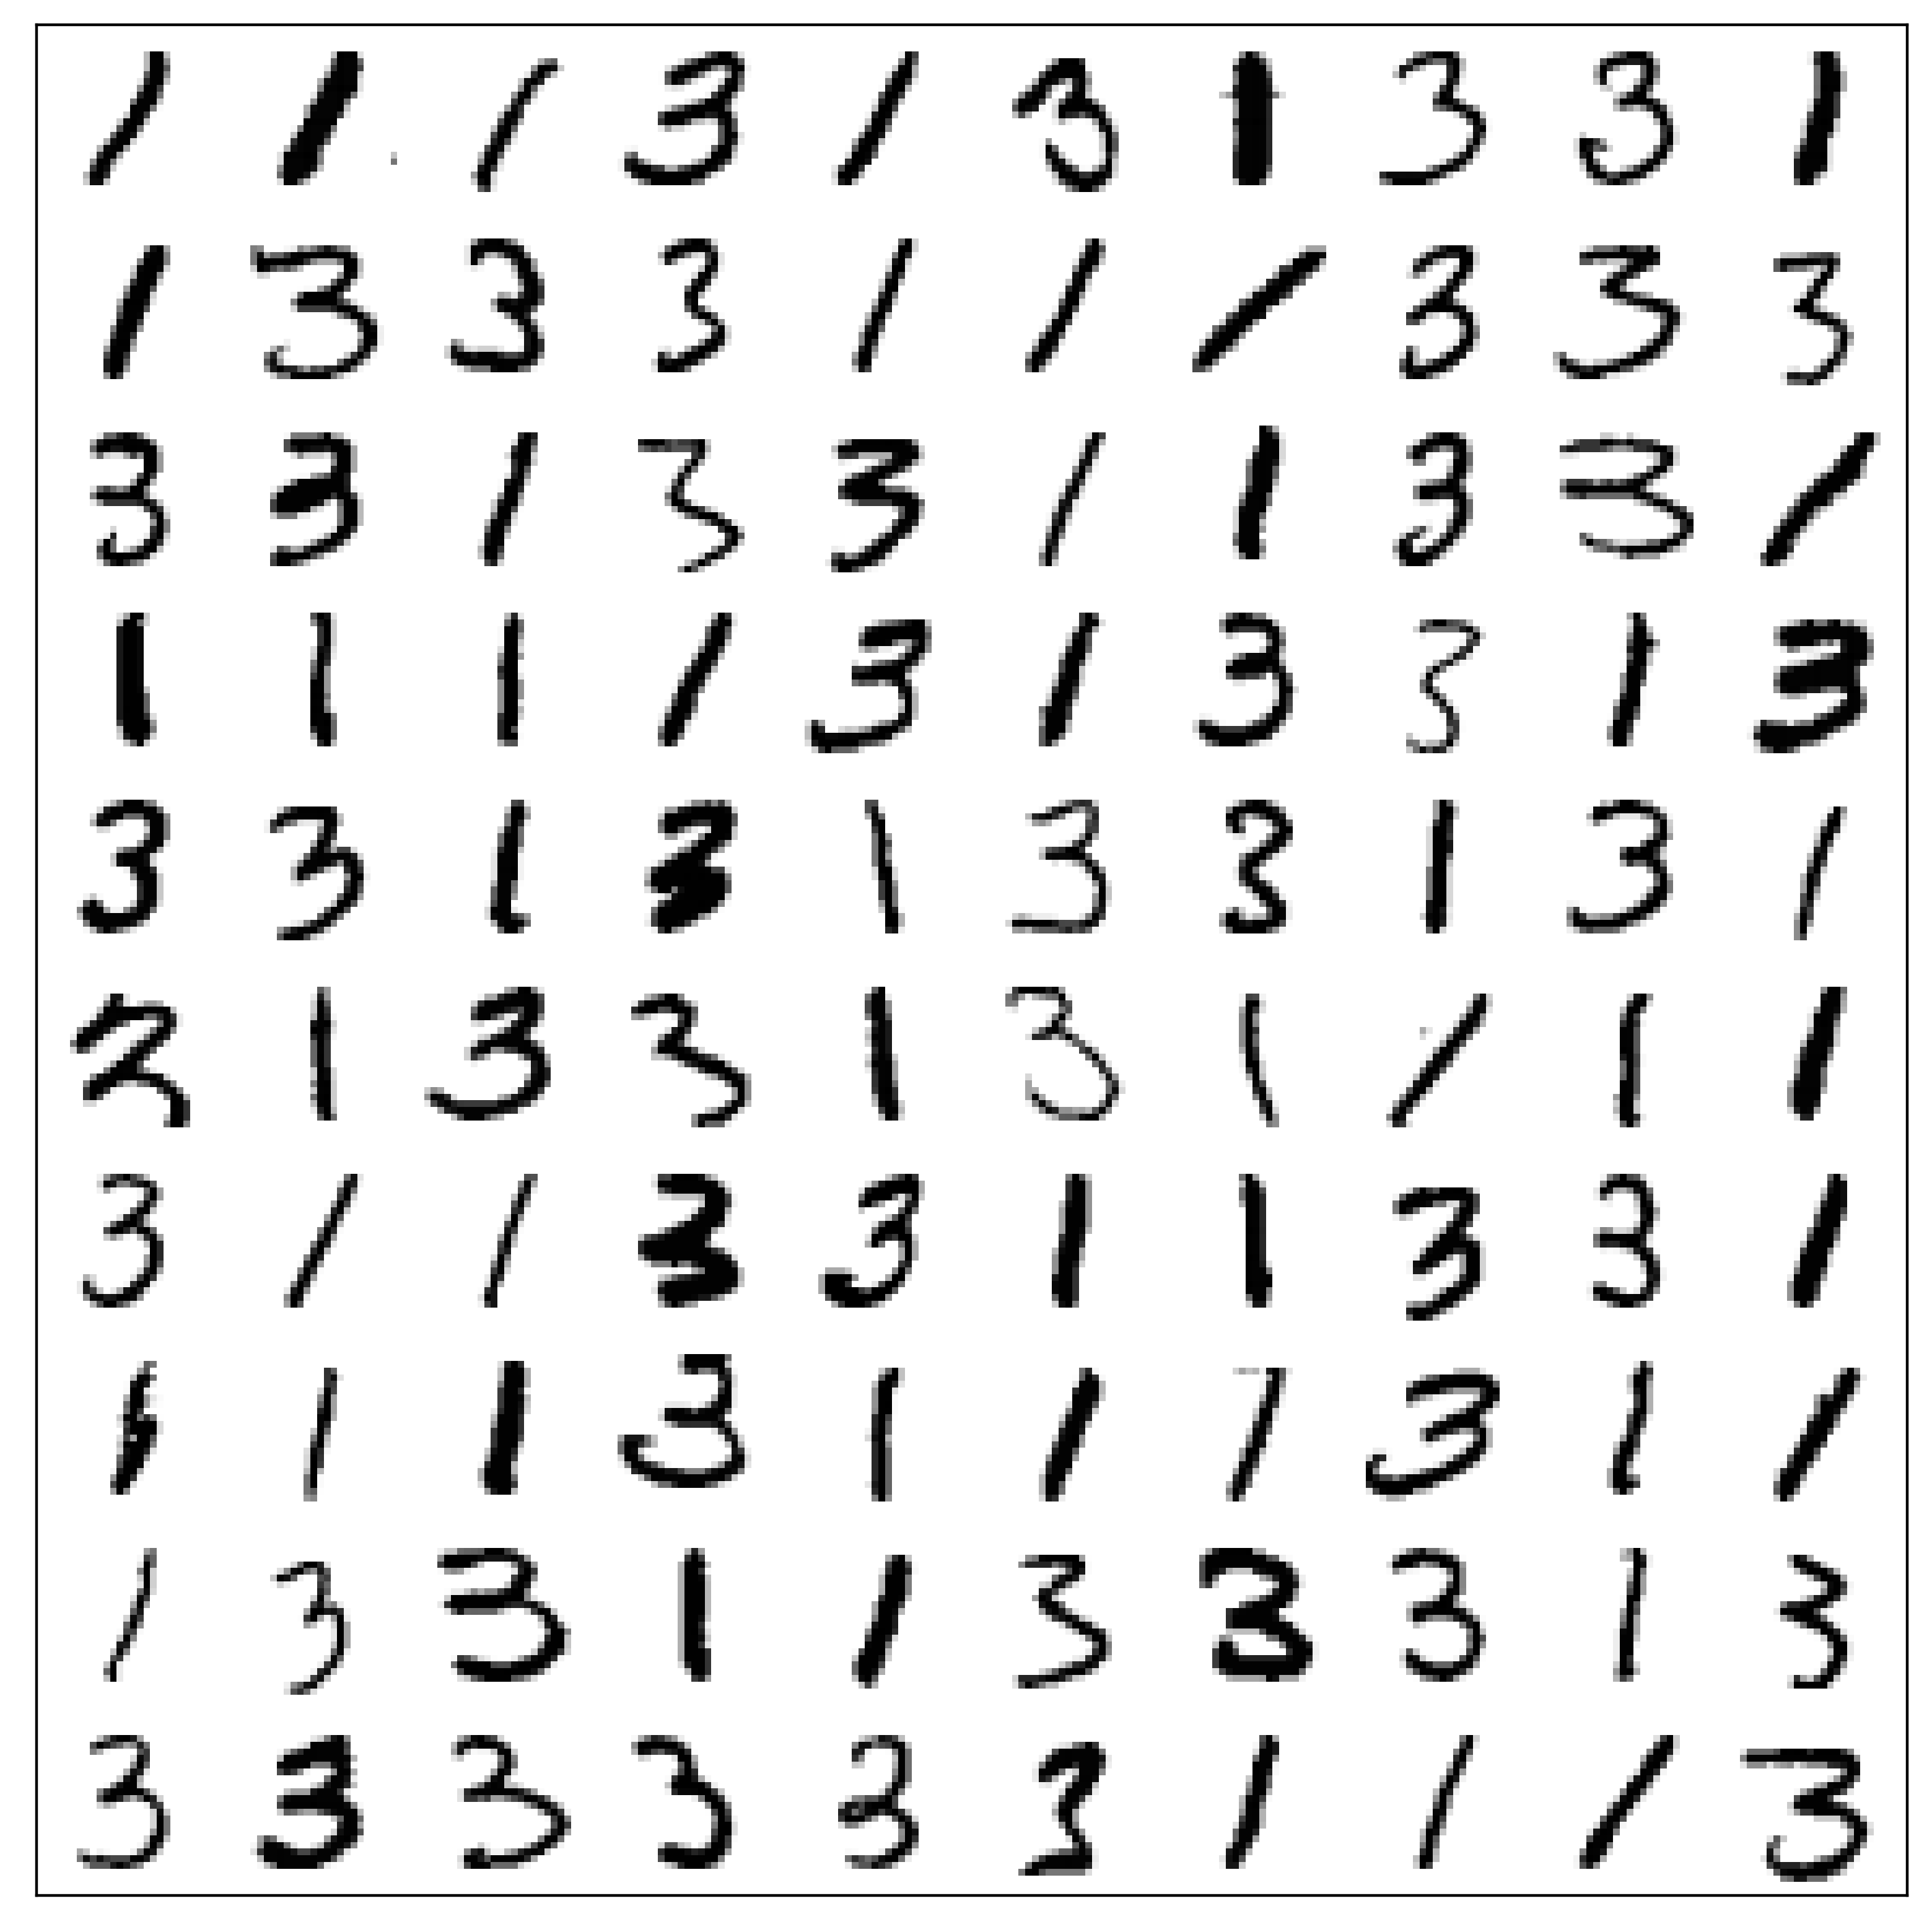
\includegraphics [width=10cm ] {o/31.png}
    \caption{"One-vs-one" batch example.}
    \label{1v1}
\end{figure}

The reason we were interested in these two modifications is that the model learns to distinguish patterns by ranking the response to those patterns among neurons, and then reinforcing the synapses of the one that responded the most.
So, in the case of "monotype" batches (figure \ref{monotype}), this could mean an increased sensibility to differences among different writings of the same digits;
for example the number 4 is handwritten either with a closed loop, as seen in the font of this document, of without the upper closed loop.
Such differences, and more subtle ones could be picked up by such a modification.
The other modification, making use of "one-vs-one" batches (figure \ref{1v1}), is interesting for a different reason:
It could lead to a better differentiation between each two digits, by confronting them through a single batch.
\todo[inline]{var vedere i risultati in questo caso}

\section{Exponential decay over time}

This is the first of two modifications inspired by the long established model for the visual cortex:
the BCM algorithm.
If we confront the original BCM equation (equation \ref{bcm})

\begin{equation}
    \frac{dW_{ij}}{dt} = \phi(h_i)x_{j} - \epsilon W_{ij}
    \label{bcm}
\end{equation}

Where $W_{ij}$ is the i-th synapses strength of the j-th hidden neuron, $\phi$ is a function of the postsynaptic activity $h_i$ that has negative value under a certain threshold and positive above, $x_{j}$ is the activation of the j-th input neuron and $\epsilon$ is a positive decay constant, we can see some similarity with our main formula (\ref{main}).
In the first, modification, is added the decay term $-\epsilon W_i$ to the main equation of the algorithm:

\begin{equation}\label{099}
    \tau_L \frac{dW_{ij}}{dt} = g(h_i)(R^p v_i - \braket{\textbf{W,v}}_i W_{ij} ) -\epsilon W_{ij}
\end{equation}

The value used for $\epsilon$ was 0.05. \todo[inline]{con altri valori che cosa si ottiene?}

\subsection{Accuracy of prediction}

\begin{table}[h!]
  \begin{center}
    \begin{tabular}{c|c} % <-- Alignments: 1st column left, 2nd middle and 3rd right, with vertical lines in between
      \textbf{Method} & \textbf{Percentage score}\\
      \hline
      Random forest & 91.6  ± 0.2\\
      Supervised network & 86.3 ± 0.5\\
      SMV & 89.3 ± 0.2\\
    \end{tabular}
  \end{center}
  \caption{Percentual Accuracy of prediction of three supervised methods.}
  \label{decayT}
\end{table}

The algorithm performed worse with this modification, as we can see in table \ref{decayT}.

This modification follows BCM, the visual cortex theory developed in 1981.
It seems that in this case the decay brings down most synapses so that they are relatively small compared to the ones that are still visible in the visual representation.
It is interesting that in this group all digits are represented.
Furthermore, the synapses are now more similar to prototypes of digits that are surrounded by small, negative synapses values.
Examining the seemingly blank sets of synapses we can see (figure \ref{nearzero}) that the pattern that characterize our model are still there, albeit of some orders of magnitude smaller, and in some cases no convergence at all is reached.

\subsection{Visual characterization}

\begin{figure} [H]
\centering
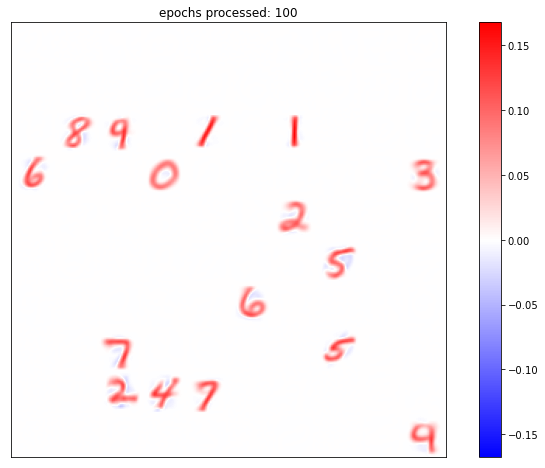
\includegraphics [width=12cm ] {h/cento.png}
\caption{Visual representation of the learned weights, with exponential decay over time.}
\label{decay}
\end{figure}

\subsection{Exponential decay over time: visual observations}

\begin{itemize}
    \item The majority of patterns are significantly weakened by the exponential decay, which could explain the worse performance on classification. Those who did not undergo this effect are more similar to prototype of digits that those of the original model.
    \item Some negative areas around them, however, are still visible.
    \item As we can see (figure \ref{nearzero}), the learned patterns are still retained, albeit very weakly. The negative values are more frequent that in those that were not greatly weakened. Some sets of weights never converged, remaining in the random state that characterized them at initialization.
\end{itemize}


\begin{figure} [H]
\centering
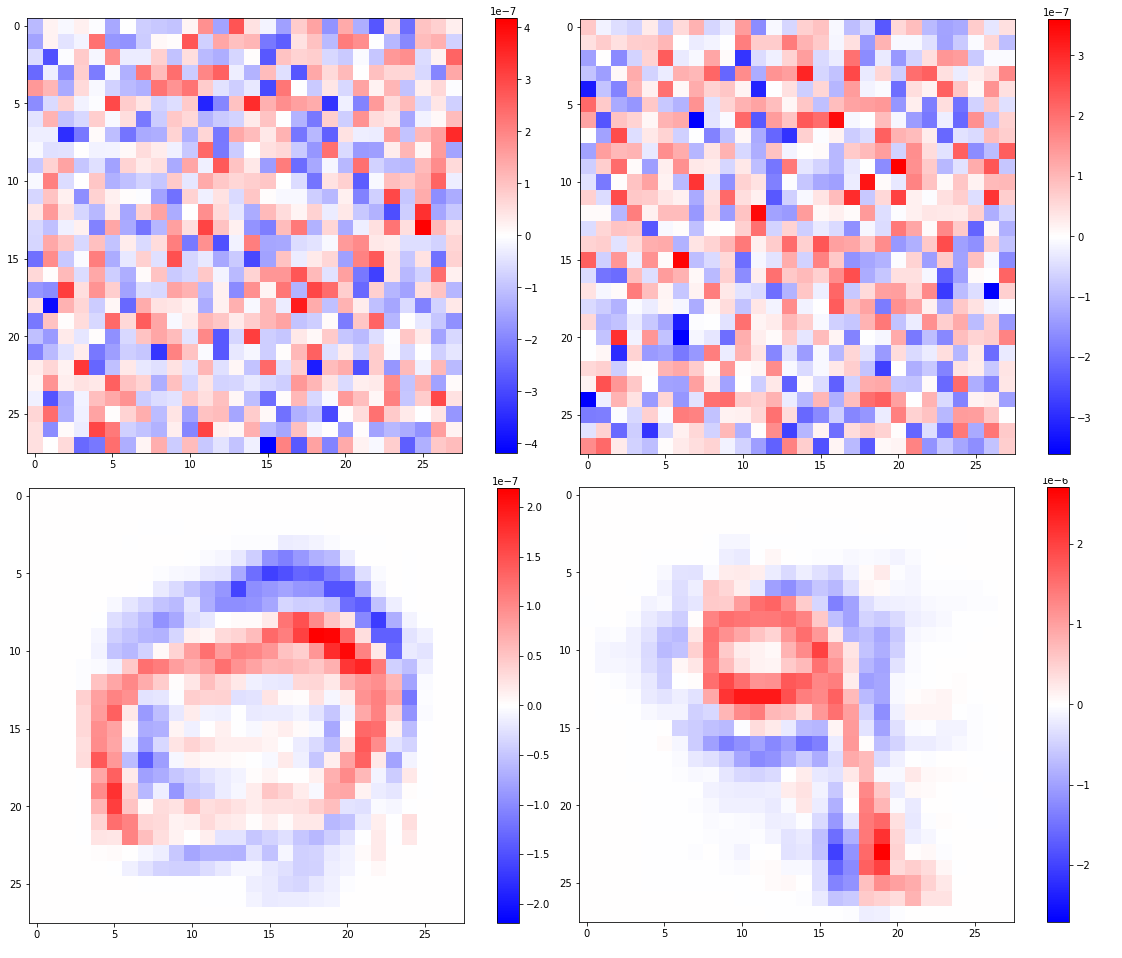
\includegraphics [width=12cm ] {h/centodue.png}
\caption{Four of the near-zero set of synapses.}
\label{nearzero}
\end{figure}

\section{Multiple neurons reinforced}

In the second BCM-inspired modification, more than one neuron undergoes Hebbian learning, so that $g$ is now equal to 1 for the k-th most activated neurons, to $-\Delta$ for the k-th most activated neuron and is null in all other cases. \todo[inline]{spiegare meglio, non è chiaro}

\subsection{Accuracy of prediction}

\begin{table}[hb!]
  \begin{center}
    \begin{tabular}{c|c} % <-- Alignments: 1st column left, 2nd middle and 3rd right, with vertical lines in between
      \textbf{Method} & \textbf{Percentual score}\\
      \hline
      Random forest & 91.7  ± 0.01\\
      Supervised network & 81.4 ± 0.4\\
      SMV & 85.7 ± 0.3\\
    \end{tabular}
  \end{center}
  \caption{Accuracy of prediction of three supervised methods.}
  \label{4tab}
\end{table}

Again, the algorithm performed worse with this modification (table \ref{4tab}).

\subsection{Visual characterization}

\begin{figure} [H]
\centering
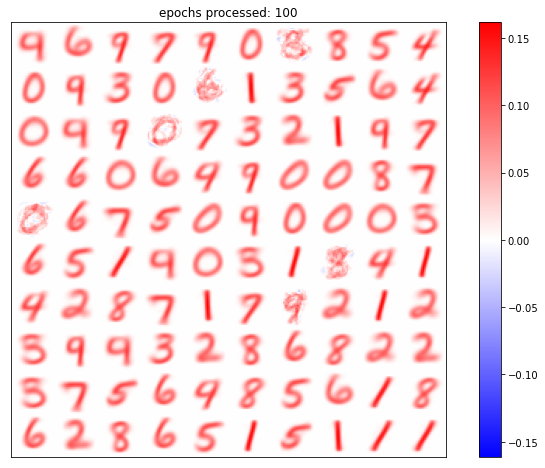
\includegraphics [width=12cm ] {h/quattrocinque.png}
\caption{Visual representation of the learned weights, with four neurons reinforced for each pattern.}
\label{multiple}
\end{figure}

\subsection{Multiple neurons reinforced: visual observations}

\begin{itemize}
    \item In this case, the Hebbian learning, now reinforcing the synapses of the four most activated neurons, almost fully compensated for the presence of anti-Hebbian learning. \todo[inline]{come cambiano i risultati con altri numeri di neuroni}
    \item Confronting this with the convergence pattern of the original algorithm, but with anti-Hebbian learning switched off  (see figure \ref{nodelta}) We observe a close similarity, except for five patterns that did not fully converged to a prototype of a digit.
    \item However, some digits seem less precise, for example in figure \ref{multiple} first row seventh column.
\end{itemize}

\chapter{Cluster analysis}

\section{Theoretical introduction}

Cluster analysis is a data classification technique that has the purpose of constructing clusters of samples that are internally homogeneous, but contain different types of samples.

In this analysis agglomerative hierarchical clustering has been used.
In this procedure, we have a definition of distance between samples that we use to get a definition of distance between clusters.
We then start joining the samples and the resulting clusters, at each step joining the two clusters that are the closest, until we group all samples in one clusters.
The results are displayed in a dendrogram, a type of graph that shows how the clusters are being made.

For example, consider the set of all inhabited continent (In the seven-continents subdivision:
North America, South America, Europe, Asia, Africa, Oceania, excluding Antarctica).
To do agglomerative hierarchical cluster analysis on this set, we would need to define a distance between continents, for example the distance between their geometric centroids, an then to define a distance between clusters of continents, for example the average distance between all elements of each cluster.
Human experience is vital in this as there's no objective best all case answer.
Then we start by measuring the distances between all starting continents, and joining in a clusters the two closest.
The final dendrogram might look like this:
(figure \ref{conte})

\todo[inline]{non è chiara la spiegazione. dettagliare meglio come funzioni il clustering agglomerativo; spiegare anche i criteri di agglomerazione fra cluster e le distanze più comuni.}

\begin{figure} [H]
\centering
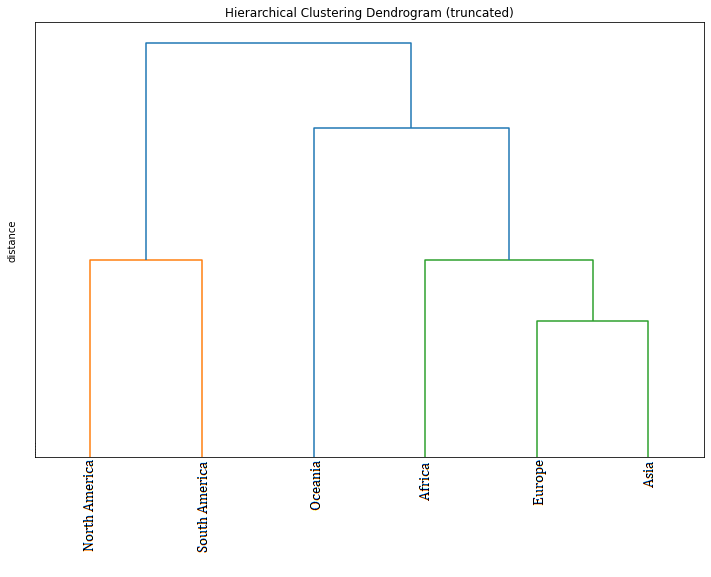
\includegraphics [width=0.7\textwidth] {o/continents.png}
\caption{Dendrogram of the continents.}
\label{conte}
\end{figure}

We can then study the graph to infer emerging information about the continents relative position from one another.
Usually in this case it is not a good idea to rely on non-human evaluation of features, because it can miss crucial details.
The most oblivious things we can infer from the graph are that Oceania is an isolated continent, but not so much that its first merge comes after all other continents have merged.

A widespread practice is the possibility of stopping the clustering at some arbitrary point and evaluating the clusters formed at that point.
Again, human evaluation is necessary.
For example, in figure \ref{conte} stopping before the merging of Oceania with the African-Eurasian cluster gives us three clusters:
the American cluster, Oceania, and the above mentioned African-Eurasian cluster.
While there is no objective way to decide where to put this threshold, it would be reasonable to say that inhabited continents are naturally divided in three clusters.

\section{Application}

An agglomerative hierarchical cluster analysis has been performed on the sets of weights of the synapses of each hidden neurons, to quantify their similarity to digits.
Since the version of the algorithm with anti-Hebbian learning switched off had better similarity to digits, it was the version used for this analysis.
(See figure \ref{nodelta})

\section{Distance definition}

In order to perform cluster analysis, a definition of distance between two set of trained synapses must be defined.
The first two definitions tried simply consider the synapses as a 784-dimensional vector:
these are euclidean distance

\begin{equation}
    d(A,B) = \sum_i (a_i-b_i)^2
\end{equation}

Where $a_i, b_i$ are the single synapses strength of sets A and B.
The resulting clusters (for an empirically determined distance threshold) can be seen in appendix B.
The second definition tried was cosine distance, i.e.
\begin{equation}
    cosine(A,B) = 1 - \frac{A \cdot B}{|A||B|}
\end{equation}

Where $|X|$ is the euclidean norm of $X$.

The resulting clusters (for an empirically determined distance threshold) can be seen in appendix C.

The final definition used, however, proved to be the best one for creating clusters containing only one digit.
The definition is taken from a 1998 paper by V. Di Gesù and V. Starovoitov on image distance definition and considers the images not as vectors but as set of points in 3-d space, with the x and y axes as pixels coordinates, and the third axis as weight associated with that synapses.
This approach has the advantage that a slight misplacement in space of weights does not cause a big difference in synapse distance.

\begin{figure} [H]
    \centering
    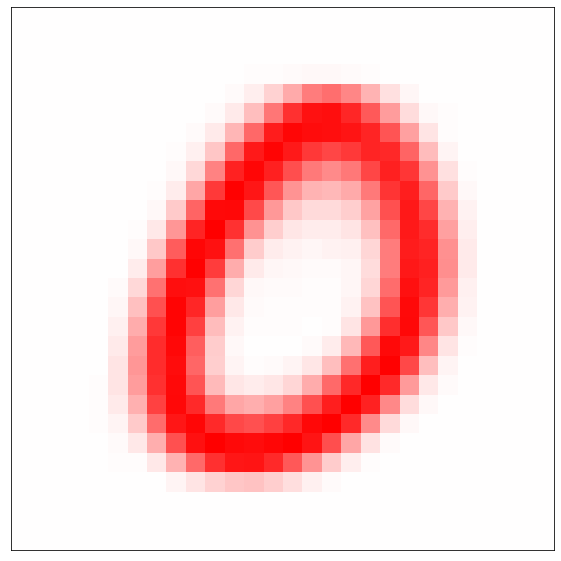
\includegraphics [width=8cm ] {o/zero.png}
    \caption{The fully trained synapses of one hidden neuron, represented as a 28 by 28 image.}
    \label{zero}
\end{figure}

\begin{figure} [H]
    \centering
    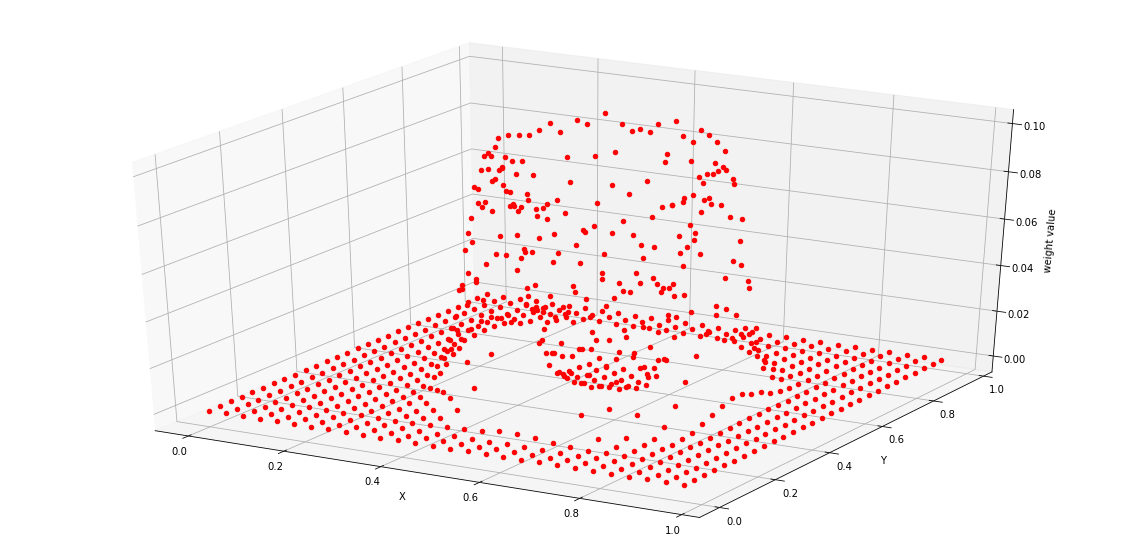
\includegraphics [width=12cm ] {o/zero_three.png}
    \caption{The same synapses represented in 3d space, with synapse strength as the z-axis.}
    \label{zero_three}
\end{figure}

The definition of distance \todo[inline]{fra cluster} is

\begin{equation}
    distance(A, B) = max(max_A(min_B(d(a,b))), max_B(min_A(d(a,b))))
\end{equation}

Where $a$ and $b$ are points belonging to set A and B respectively, and $d(a,b)$ is their euclidean distance.
The definition of distance between clusters is the average of all between-clusters element distances.

This definition proved to be the best out of others used \todo[inline]{come sono state valutate? facciamo vedere dei risultati quantitativi per i vari casi!}, as it permitted to separate the synapses in eighteen different clusters, mostly composed by only one digit.



\section{Resulting clusters from 18-clusters agglomerative hierarchical clustering}

With this definition, out of 18 clusters \todo[inline]{decisi come? perché 18 e non 17 o 19?}, 15 were formed by only one digit, 2 were formed by two digits, and only one was formed of three different digit prototypes.
All clusters can be visualized in the appendix. \todo[inline]{mettere i numeri ai cluster in modo da capire come si agglomerano}

\begin{figure} [H]
    \centering
    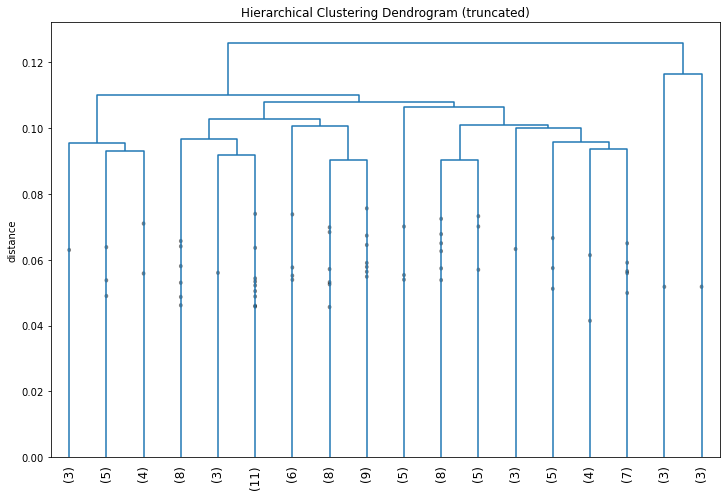
\includegraphics [width=\textwidth]{o/clustering.png}
    \caption{The resulting dendrogram. The between parenthesis number at the bottom of each line represents the number of samples in that particular cluster. Black dots represent a merge between of two clusters.}
    \label{clustering}
\end{figure}

\subsection{Observations on the resulting clusters}

\begin{itemize}
    \item The only triple digit cluster (figure \ref{910}, on the left) is composed of eights, arguably the most complicated shape and thus the least separable from the others, fives and threes that share each part of the shape with eight, especially looking at the definition of distance we gave to the algorithm.

\begin{figure} [H]
    \centering
    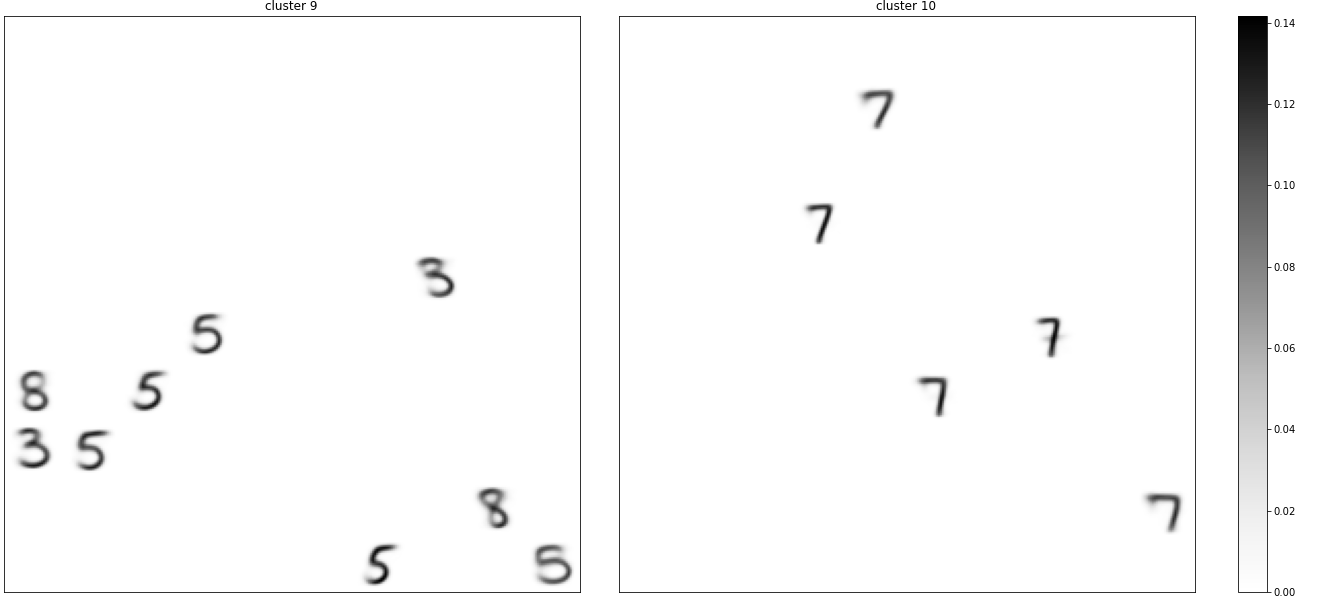
\includegraphics [width=\textwidth ] {c/h/9.png}
    \caption{}
    \label{910}
\end{figure}

    \item The two double digit clusters are composed of nines and fours, which again intuitively aren't at a great distance (figure \ref{12}) according to our definition.

\begin{figure} [H]
    \centering
    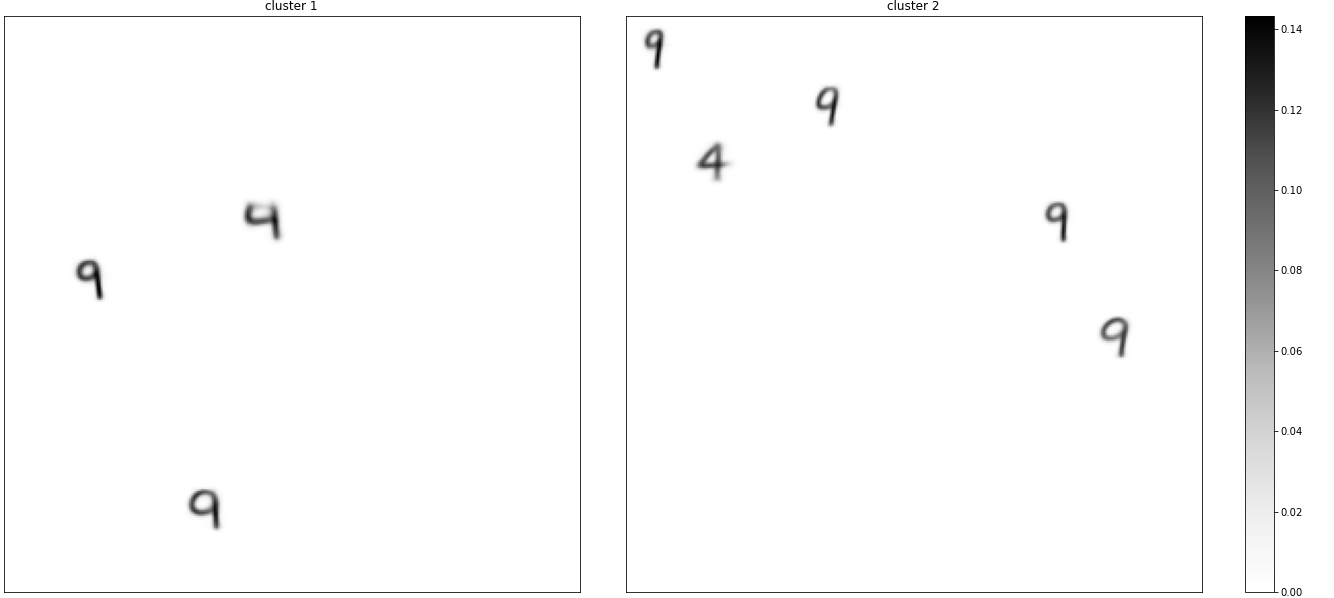
\includegraphics [width=\textwidth ] {c/h/1.png}
    \caption{}
    \label{12}
\end{figure}

    \item The two double digit clusters (figure \ref{12}) are composed of nines and fours. In cluster 2, all digits are nine but a four, which is very different from all other fours, which explains the "wrong" classification.
    \item Zeros cluster by themselves well even cutting the dendrogram higher.

    \item Clusters 11 and 12 (figure \ref{1112}) make evident the difference between the two types of two prototypes: with and without loop.

\begin{figure} [H]
    \centering
    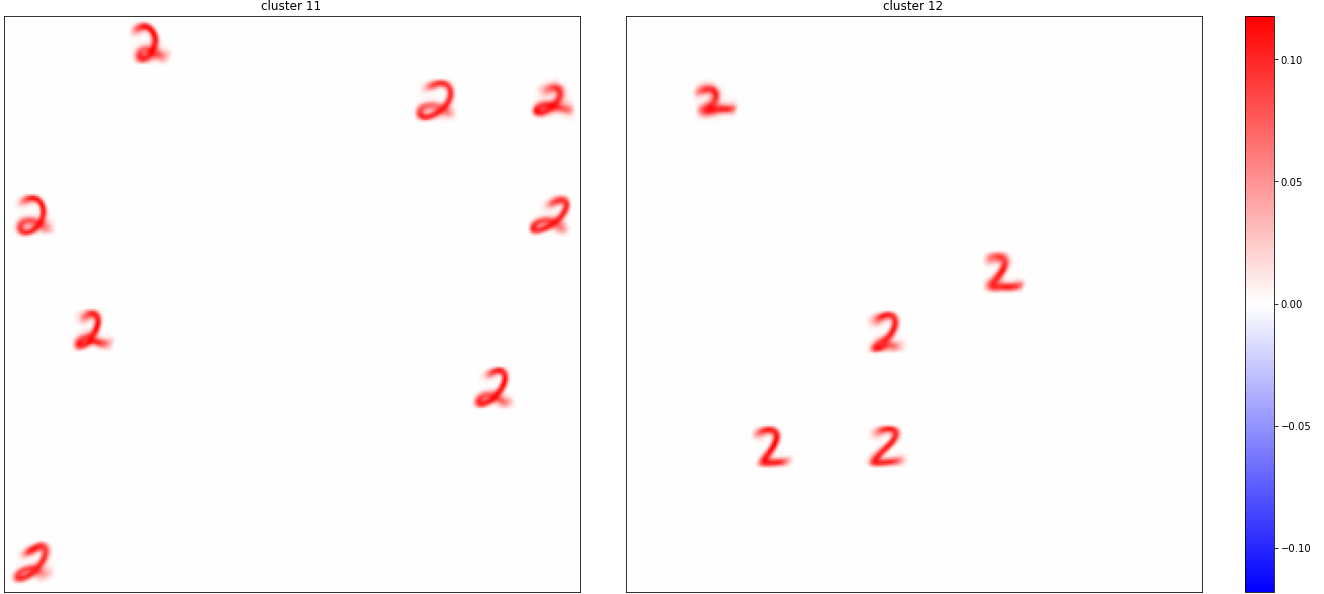
\includegraphics [width=\textwidth ] {c/h/11.png}
    \caption{}
    \label{1112}
\end{figure}

    \item Clusters 17 and 18 joined late and their resulting cluster (we can see that one groups ones which are tilted, the other ones that are not) was the last joining all other digits. (see figure \ref{final})
\end{itemize}

\begin{figure} [H]
    \centering
    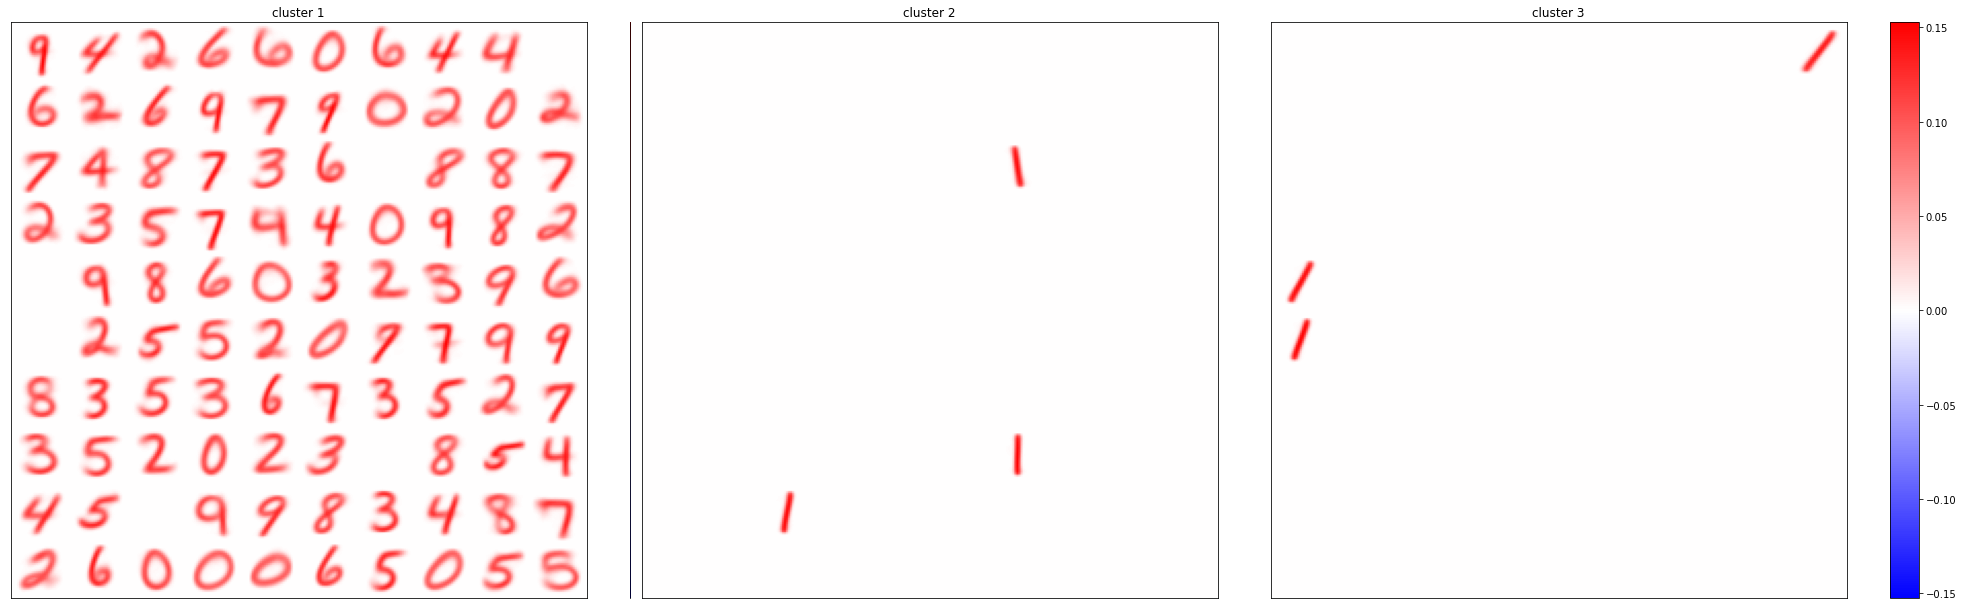
\includegraphics  [width=\textwidth]  {c/h/final1.png}
    \caption{The three final clusters merging. The middle and right cluster correspond to clusters 17 and 18 of the 18-clusters subdivision.}
    \label{final}
\end{figure}

\chapter{Conclusions}

Considering first of all the results obtained in table \ref{bbb}, one must not be surprised that the results are much lower than those in the original paper by Hopfield and Krotov (in which a 1.46\% accuracy is reached \todo[inline]{sicuro del numero?}), as the number of both hidden neurons and processed epochs is much smaller (2000 hidden units and 1000 epochs vs 100 hidden units and 100 epochs), which greatly reduces both computational times and accuracy of prediction. \todo[inline]{sarebbe da far vedere un confronto corrispondente, non ha senso parlare dei risultati del paper}

The emerging patterns among synapses strength are of particular interest.
Unlike in the case of more traditional, backpropagation based networks, they are interpretable by the human eye as similar to prototypes of the input samples, their utility goes beyond that.
A common occurrence observed (see figure \ref{heatmap}) is a positive digit surrounded by a negative border, a common practice among human designed networks that reduces the possibility of confusion between digits.
Another observed behaviour is a set of hidden neuron synapses in which it is possible to recognize two numbers:
one "drawn" in positive synapses strengths, and the other in negative.
These values might reveal very useful in distinguishing between two classes of digits, as they respond with a positive activation for one digit and a negative one for the other.

The modification that gave us one of the most interesting result is switching off explicit anti-Hebbian learning.
First off, note that there still is a competition between patterns, as only the most activated one gets reinforced at all, but every neuron is still bound by the fact that every set of synapses must converge to a sphere.
All the synapses are now positive, as it is to be expected from the positive reinforcement of our model.
They also resemble only prototypes of the training database.
We lose the negative border effect and the superimposition of two digits previously discussed.
However, we can more easily recognize the digits prototypes.
A characteristic of these positive patterns is also consistency, as they presented themselves in the two modifications of the model inspired to BCM learning, the one with exponential over-time decay of weights and the one with multiple neurons reinforced.
Also, varying the hyperparameters of this model did not changed the existing pattern by a significant amount.
We did not observe a significant change in accuracy either, however we know from the paper by Hopfield and Krotov that when working with their increased number of epochs and hidden neurons the difference is significative (switching off anti-Hebbian learning lowers the accuracy from 98.54\% to 97.98\%).

\chapter{Acknowledgements}
This document is the culmination of five years of work.
It was written thanks to the support of these people.

First and foremost, thank you, professor Giampieri:
without your help and patience I could not have written this thesis.
I firmly believe that if everybody followed your standards on code documentation, we'd have flying cars by now.

Thanks to my family.
Dad, you were there when I needed it the most.
I live by the strict principle of your education:
always do whatever I want.
Mom, you taught me to never take myself too seriously.
I'd like to tell you to go fetch your nose, clown.
Teo, you remembered me that life is not a prison.

Thank you to my friends who accompanied me through these five years:
Alessandra, Chiara, Elia, Gianpiero, Irina, Laura, Lorenzo B., Lorenzo L., Luca, Luigi, Monica, Olly, Riccardo, Sara and all the others.
Irina, you've been a caring friend;
It means so much for me.
Monica, you got me out of a bad place;
I can only hope of giving back one tenth of what you gave to me.
Lorenzo B., when I was alone you were there for me, can a friend ask for more?
Lorenzo L. and Chiara, your enthusiasm in getting exploited by the pro loco of my hometown has been inspiring.
Luigi, you answered five years of questions, and appreciated with me the fine art form of memes.
Olly, you've been a real friend across any political or religious barrier.

Thank you to ER.GO. and the Occhialini foundation, which gave me the means to be here, and to University of Bologna for the SAP service, which lighted a candle when I was in darkness.

For all these reasons and one thousand more, thank you all.

\bibliography{bibliography}

\appendix

\chapter{Haussdorf distance Cluster analysis: resulting clusters}

The 18 clusters obtained with the definition of distance as

\begin{equation}
    distance(A, B) = max(max_A(min_B(d(a,b))), max_B(min_A(d(a,b))))
\end{equation}

Where $a$ and $b$ are points belonging to set A and B respectively, $d(a,b)$ is their euclidean distance, and set A and B are composed of points in 3d space with the first two coordinates as pixel coordinates and the third coordinate as synapse strength.

The linkage method used was to take the average of distances between members of the two clusters.

\begin{figure} [H]
    \centering
    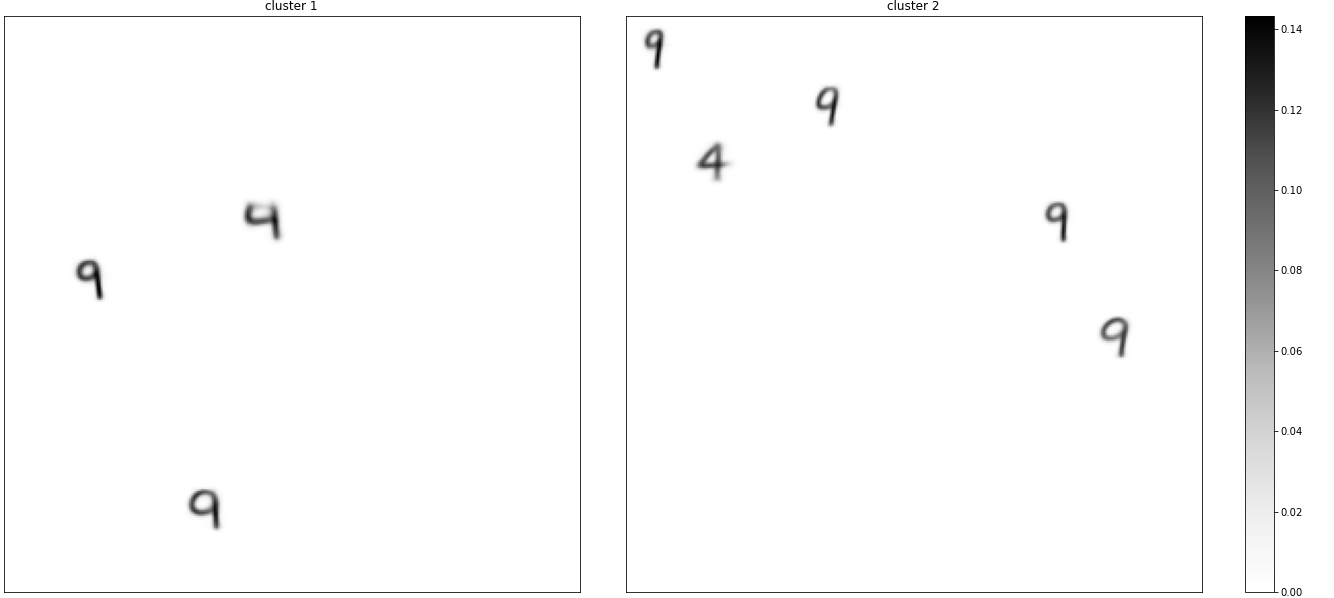
\includegraphics [width=\textwidth ] {c/h/1.png}
    \caption{}
\end{figure}

\begin{figure} [H]
    \centering
    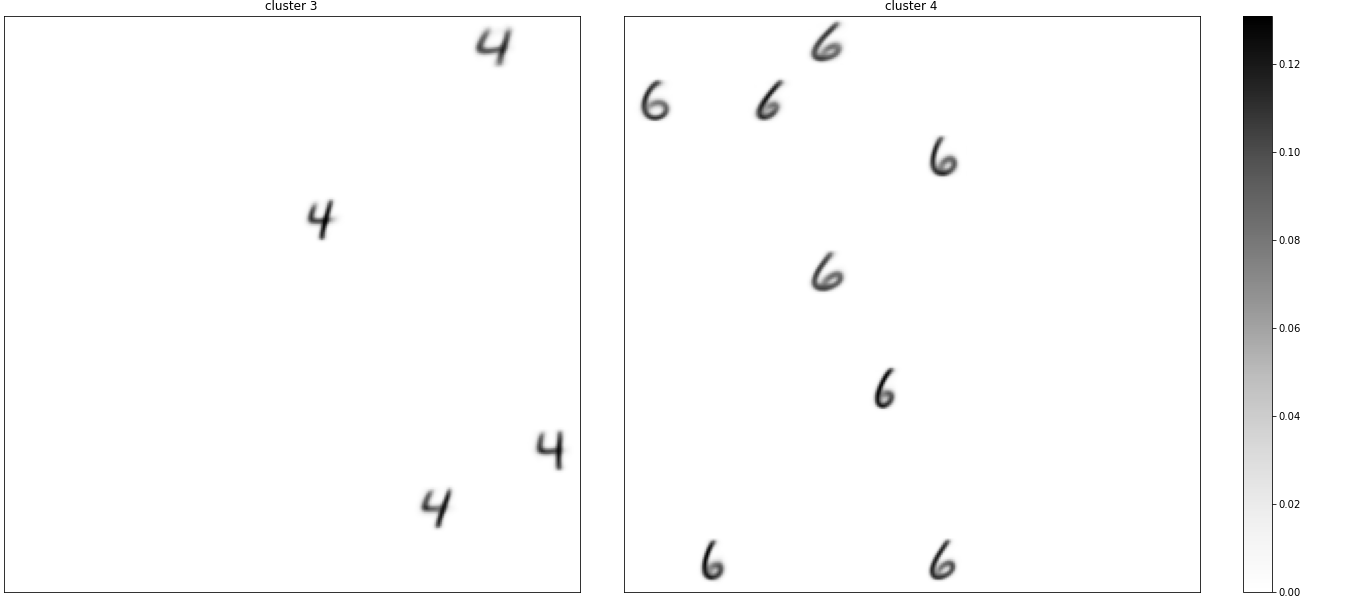
\includegraphics [width=\textwidth ] {c/h/3.png}
    \caption{}
\end{figure}

\begin{figure} [H]
    \centering
    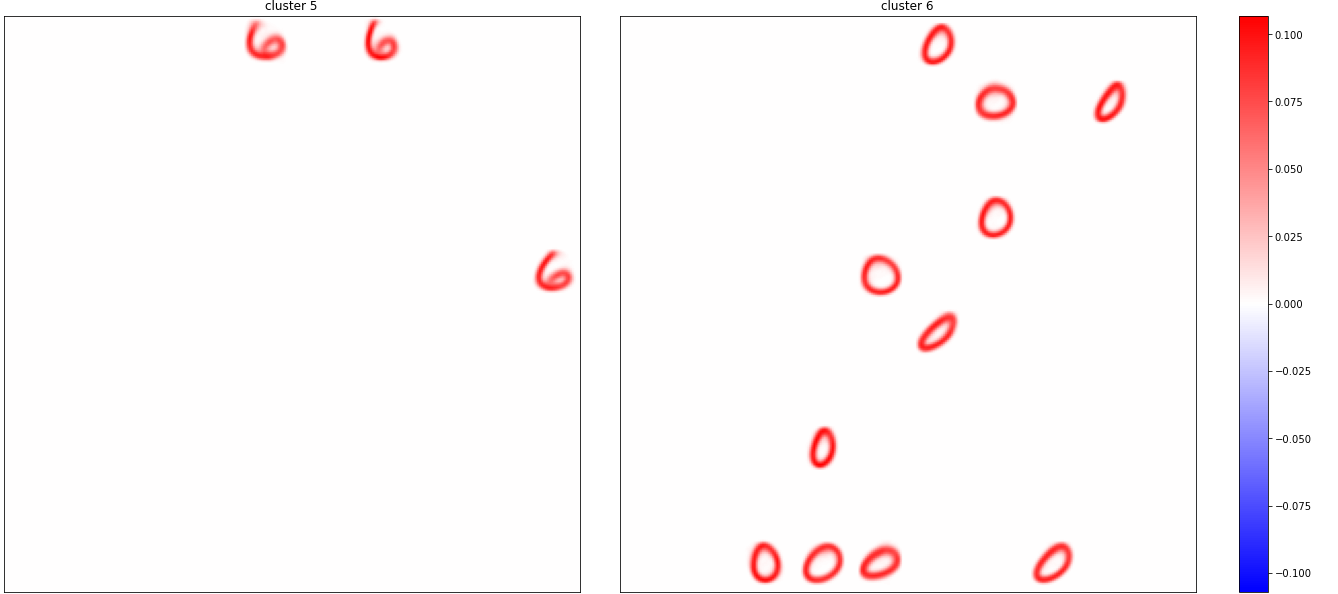
\includegraphics [width=\textwidth ] {c/h/5.png}
    \caption{}
\end{figure}

\begin{figure} [H]
    \centering
    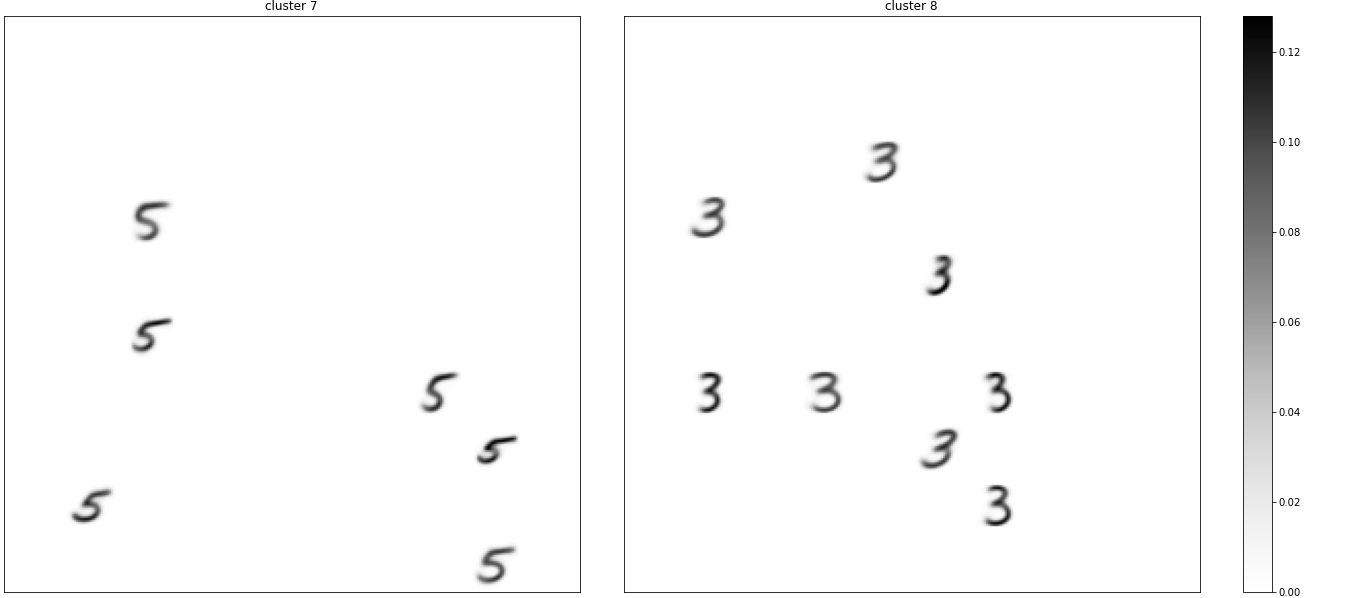
\includegraphics [width=\textwidth ] {c/h/7.png}
    \caption{}
\end{figure}

\begin{figure} [H]
    \centering
    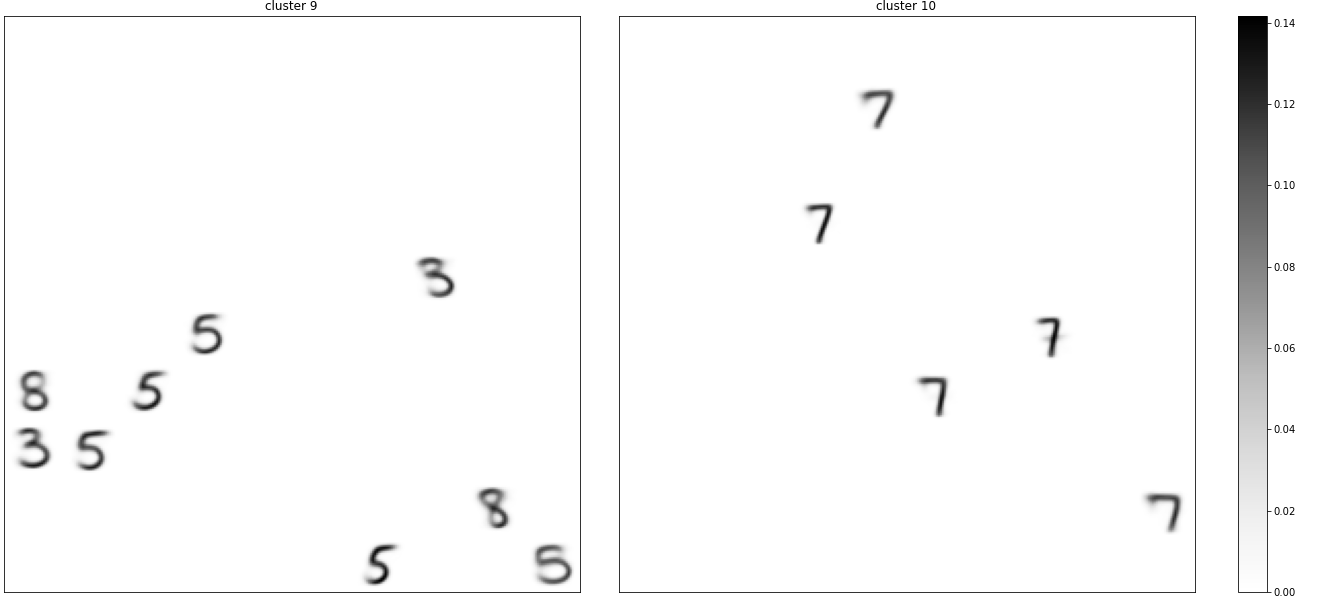
\includegraphics [width=\textwidth ] {c/h/9.png}
    \caption{}
\end{figure}

\begin{figure} [H]
    \centering
    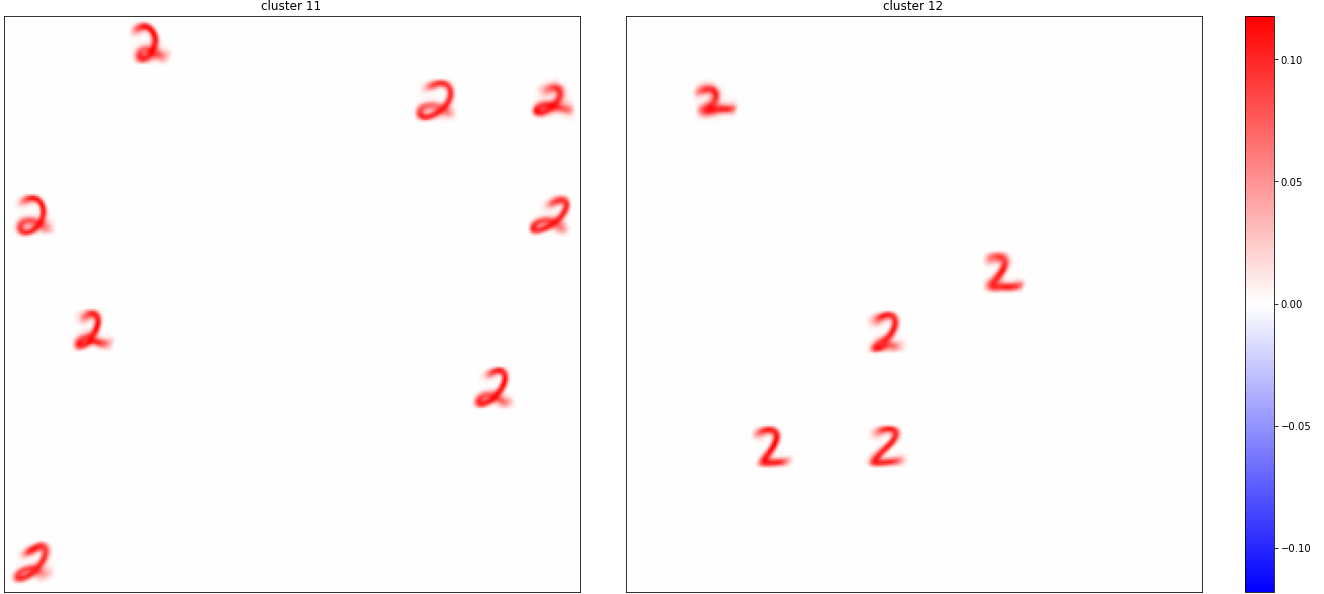
\includegraphics [width=\textwidth ] {c/h/11.png}
    \caption{}
\end{figure}

\begin{figure} [H]
    \centering
    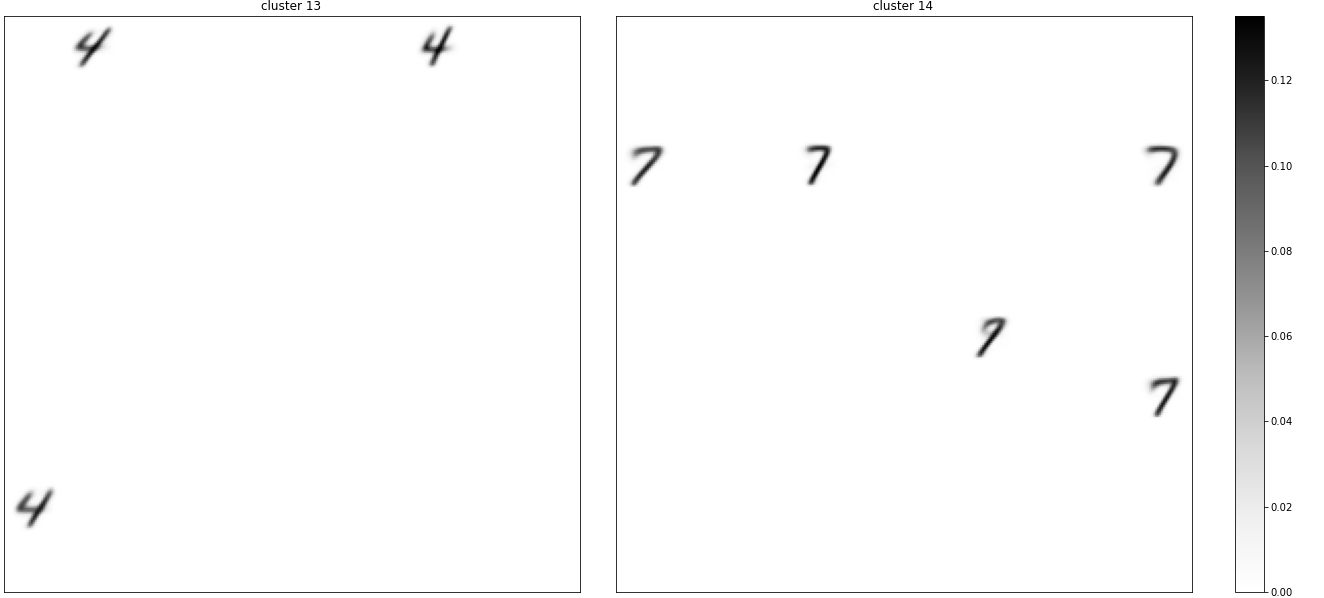
\includegraphics [width=\textwidth ] {c/h/13.png}
    \caption{}
\end{figure}

\begin{figure} [H]
    \centering
    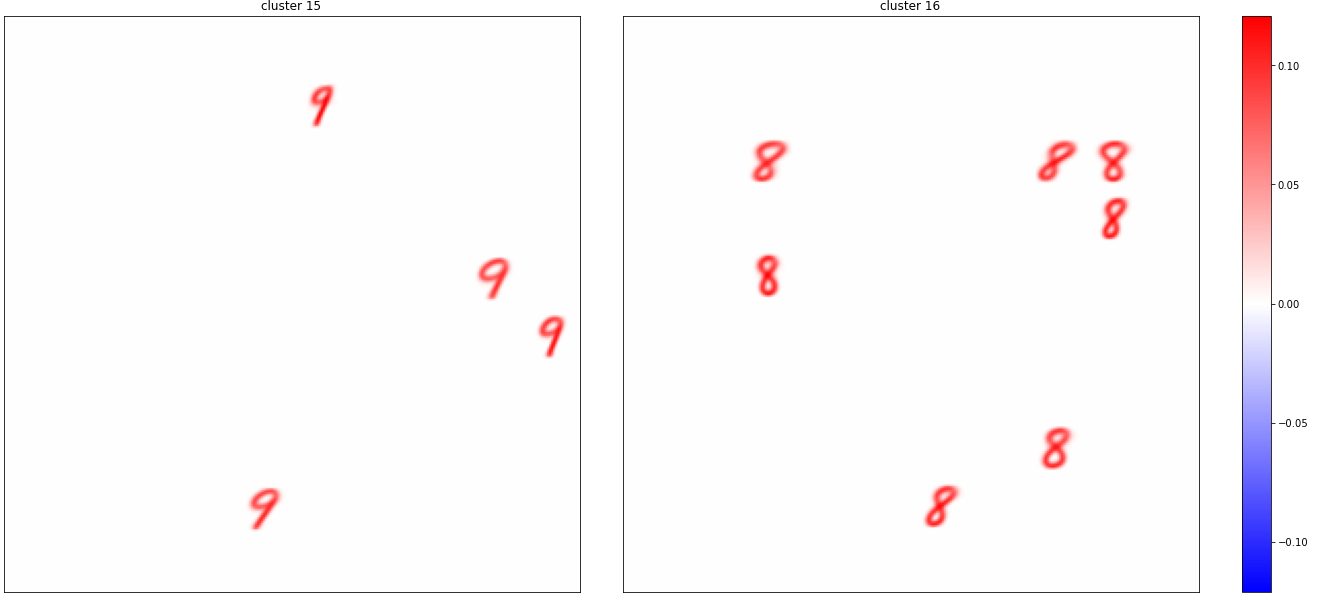
\includegraphics [width=\textwidth ] {c/h/15.png}
    \caption{}
\end{figure}

\begin{figure} [H]
    \centering
    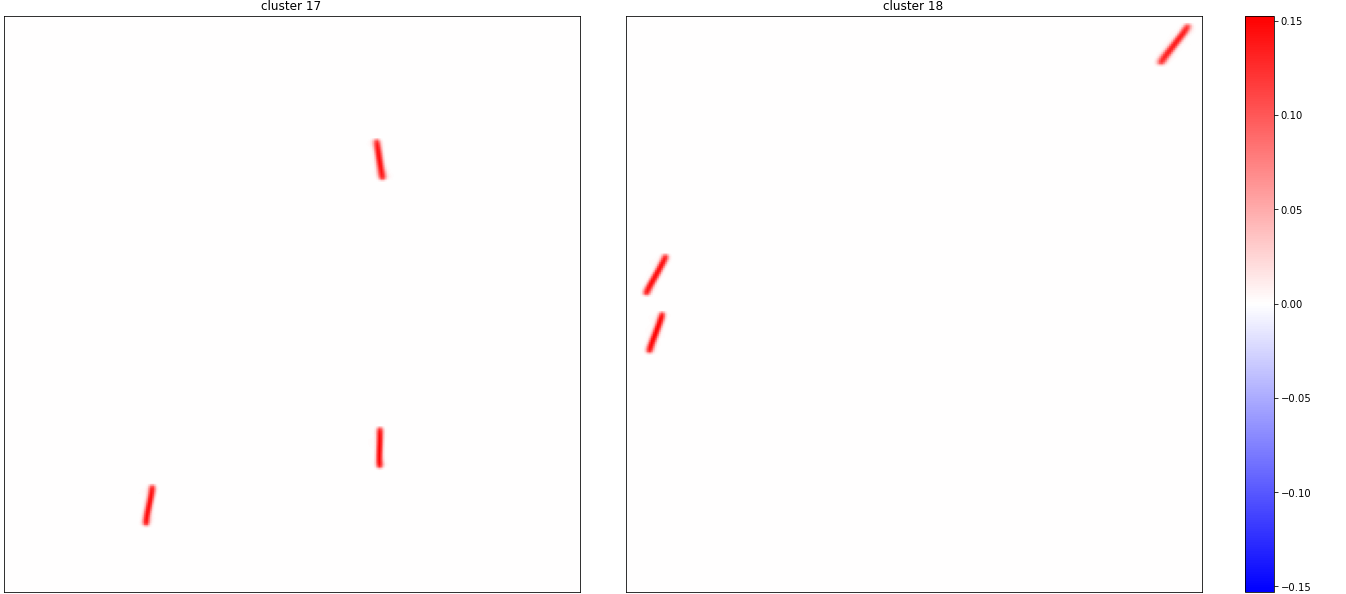
\includegraphics [width=\textwidth ] {c/h/17.png}
    \caption{}
\end{figure}

\chapter{Euclidean distance clusters analysis: resulting clusters}

The definition of distance used is the normal euclidean distance

\begin{equation}
    d(A,B) = \sum_i (a_i - b_i)^2
\end{equation}

Where $a_i, b_i$ are the single synapses strenght of sets A and B.

The method of linkage used is the Ward method, in wich the distance between two clusters is defined as the internal variance of the resulting cluster.

\begin{figure} [H]
    \centering
    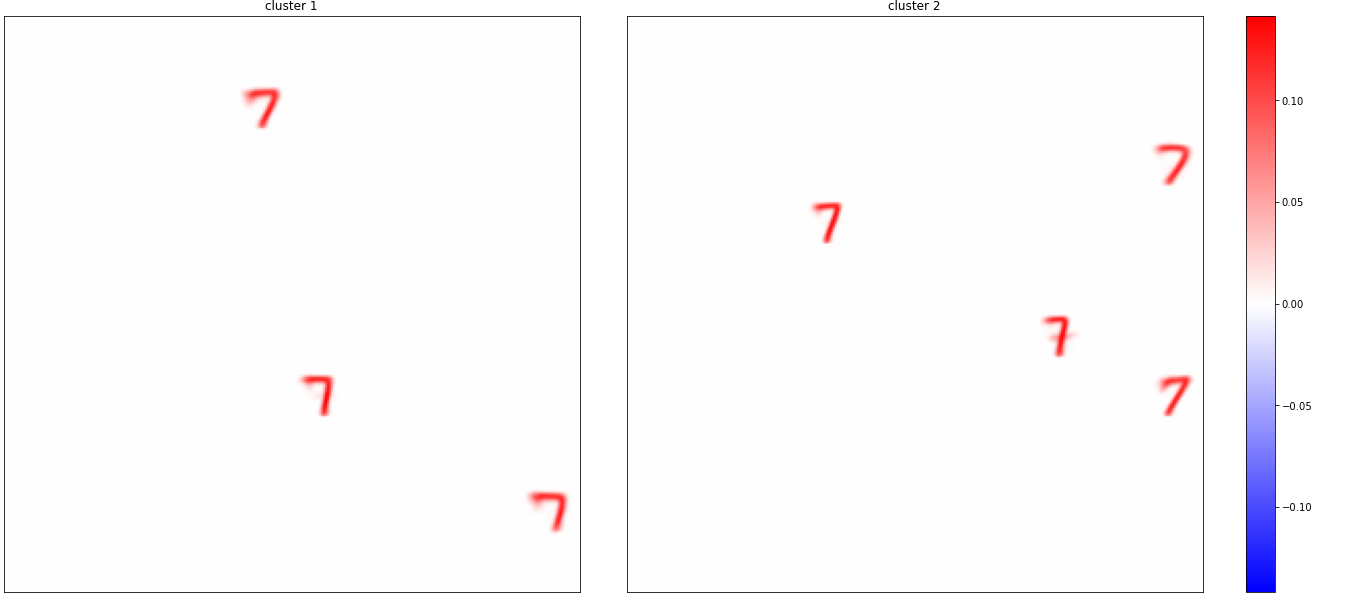
\includegraphics [width=\textwidth ] {c/e/1.png}
    \caption{}
\end{figure}

\begin{figure} [H]
    \centering
    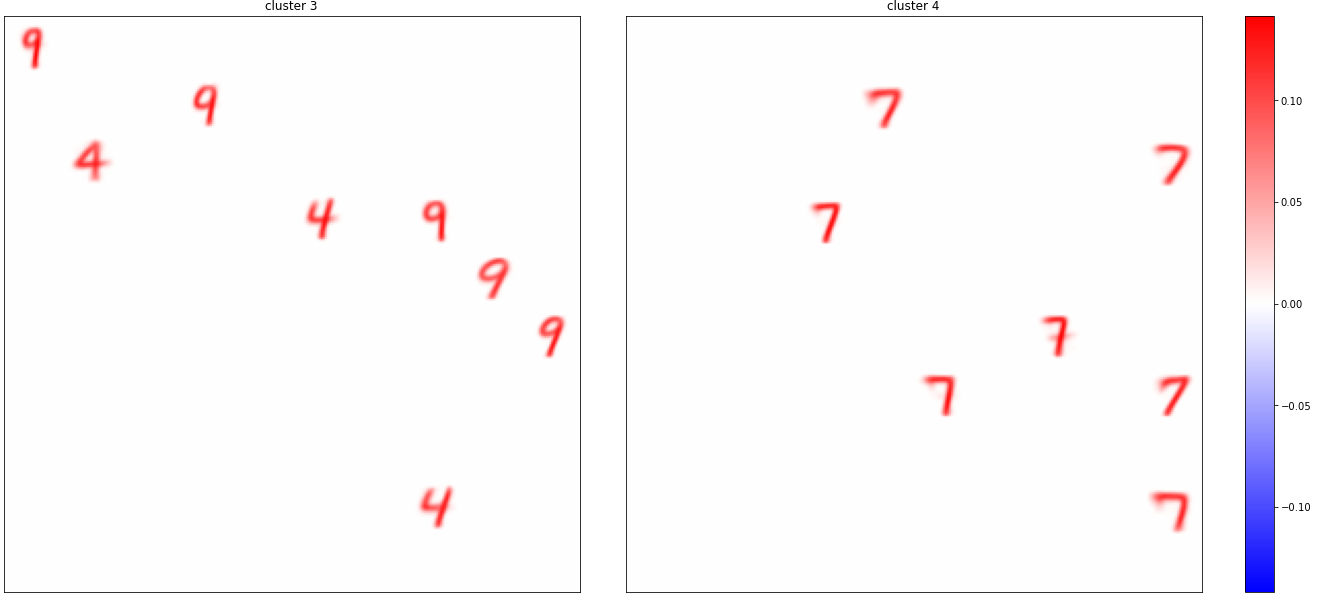
\includegraphics [width=\textwidth ] {c/e/3.png}
    \caption{}
\end{figure}

\begin{figure} [H]
    \centering
    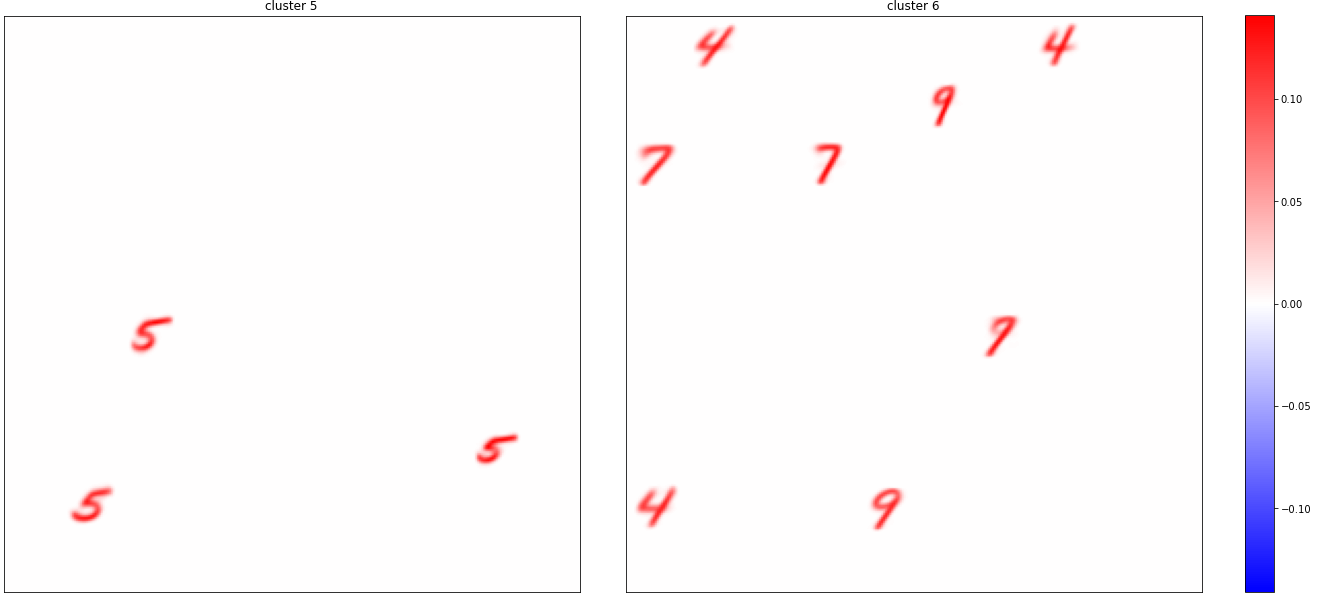
\includegraphics [width=\textwidth ] {c/e/5.png}
    \caption{}
\end{figure}

\begin{figure} [H]
    \centering
    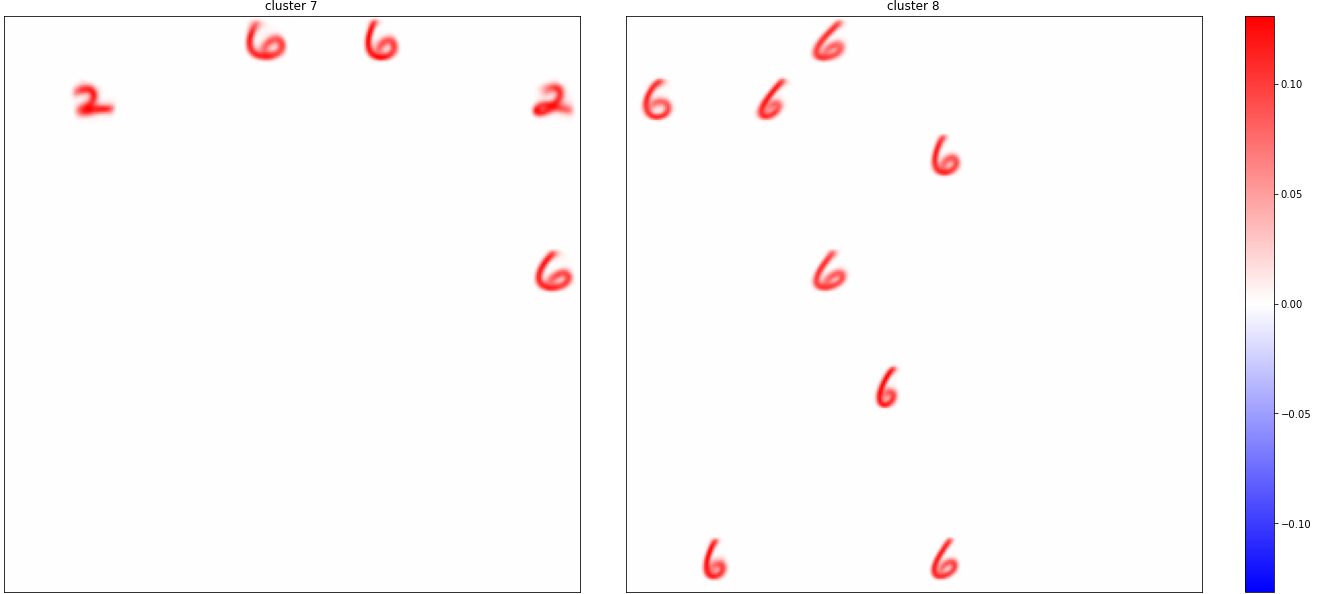
\includegraphics [width=\textwidth ] {c/e/7.png}
    \caption{}
\end{figure}

\begin{figure} [H]
    \centering
    \includegraphics [width=\textwidth ] {c/e/9.png}
    \caption{}
\end{figure}

\begin{figure} [H]
    \centering
    \includegraphics [width=\textwidth ] {c/e/11.png}
    \caption{}
\end{figure}

\begin{figure} [H]
    \centering
    \includegraphics [width=\textwidth ] {c/e/13.png}
    \caption{}
\end{figure}

\chapter{Cosine distance cluster analysis: resulting clusters}

The definition of cosine distance is

\begin{equation}
    cosine(A,B) = 1 - \frac{A \cdot B}{|A||B|}
\end{equation}

Where A and B are vectors containing our synapses strenghts.

The linkage method used was to take the average of distances between members of the two clusters.

\begin{figure} [H]
    \centering
    \includegraphics [width=\textwidth ] {c/c/1.png}
    \caption{}
\end{figure}

\begin{figure} [H]
    \centering
    \includegraphics [width=\textwidth ] {c/c/3.png}
    \caption{}
\end{figure}
\begin{figure} [H]
    \centering
    \includegraphics [width=\textwidth ] {c/c/5.png}
    \caption{}
\end{figure}\begin{figure} [H]
    \centering
    \includegraphics [width=\textwidth ] {c/c/7.png}
    \caption{}
\end{figure}\begin{figure} [H]
    \centering
    \includegraphics [width=\textwidth ] {c/c/9.png}
    \caption{}
\end{figure}
\begin{figure} [H]
    \centering
    \includegraphics [width=\textwidth ] {c/c/11.png}
    \caption{}
\end{figure}
\end{document}
